\chapter{Descripción}\label{chapter04}

\section{Requerimientos}\label{sec:requerimientos}
A continuación se presentan los requerimientos de la solución, organizados en dos categorías: requerimientos funcionales y no funcionales. Los requerimientos funcionales representan las operaciones y servicios que la plataforma debe ofrecer al usuario final, mientras que los no funcionales establecen criterios de calidad que condicionan la forma en que el sistema debe operar \parencite{ieee2008}.

SmartStocker está diseñado para asistir a pequeños y medianos establecimientos gastronómicos en la gestión de su inventario. A partir de la integración con plataformas de ventas y el análisis de datos históricos mediante técnicas de Machine Learning, el sistema proyecta la demanda futura, calcula el stock necesario y genera alertas tempranas para evitar pérdidas por desabastecimiento o exceso. Asimismo, provee un tablero con métricas relevantes y permite al usuario interactuar con el modelo de predicción para ajustarlo a la realidad de su negocio mediante feedback.

\subsection{Requerimientos funcionales}\label{sec:requerimientos-funcionales}
Los requerimientos funcionales describen las acciones observables que el sistema debe llevar a cabo para satisfacer las necesidades del usuario \parencite{ieee2008}.
\begin{enumerate}[label=\textbf{RF\arabic*}, leftmargin=2.5cm]
    \item El sistema debe permitir el alta de cuentas de restaurantes, con autenticación segura mediante correo electrónico y contraseña.
    \item El sistema debe permitir registrar, modificar y eliminar productos gastronómicos, vinculados con los insumos que los componen.
    \item El sistema debe facilitar la administración de inventario, incluyendo actualización de cantidades disponibles y definición de umbrales mínimos de stock.
    \item El sistema debe conectarse con plataformas de delivery en CABA (por ejemplo, PedidosYa) para importar datos de ventas en tiempo real.
    \item El sistema debe permitir la carga manual de datos históricos de ventas a través de archivos en formato \texttt{.csv} o \texttt{.xlsx}.
    \item El sistema debe ejecutar predicciones de ventas que sean basadas en modelos de Machine Learning, considerando tanto información histórica como variables externas (clima, feriados, días de la semana).
    \item El sistema debe calcular automáticamente la cantidad de inventario recomendada según los resultados de las predicciones generadas.
    \item El sistema debe emitir alertas cuando un insumo se encuentre por debajo del nivel mínimo configurado por el usuario.
    \item El sistema debe permitir al usuario proporcionar retroalimentación respecto a las predicciones, incorporando estos datos para el ajuste del modelo.
\end{enumerate}

\subsection{Requerimientos no funcionales}\label{sec:requerimientos-no-funcionales}
Los requerimientos no funcionales especifican condiciones de calidad y restricciones técnicas que determinan cómo debe operar la solución, más allá de las funciones explícitas que ofrece \parencite{ieee2008}.
\begin{enumerate}[label=\textbf{RNF\arabic*}, leftmargin=2.8cm]
    \item La interfaz debe ser adaptable (responsive) para asegurar su correcto uso en computadoras de escritorio, tablets y dispositivos móviles.
    \item La aplicación debe garantizar disponibilidad continua ($24 \times 7$) para el acceso a predicciones, métricas e informes en cualquier momento.
    \item El sistema debe ser compatible con los navegadores más utilizados (Google Chrome, Mozilla Firefox, Microsoft Edge y Safari) en sus versiones estables recientes.
    \item La infraestructura debe poder escalar automáticamente para soportar un crecimiento sostenido de usuarios sin afectar el rendimiento.
    \item El sistema debe desplegarse en una plataforma en la nube (por ejemplo, AWS Amplify) que garantice al menos un 99\% de disponibilidad mensual.
\end{enumerate}

\section{Diagramas}\label{sec:diagramas}

Para comprender de manera clara la interacción entre los usuarios y el sistema, así como el flujo de los procesos internos, se emplean diferentes tipos de diagramas. Estas representaciones gráficas permiten comunicar de forma visual los requerimientos, las funcionalidades y la lógica de operación de la aplicación, favoreciendo la comprensión tanto de aspectos funcionales como de diseño \parencite{booch2005uml}. 

A continuación, se detallan los posibles flujos funcionales que se encuentran disponibles en SmartStocker.

\subsection{Diagramas de Casos de Uso}\label{sec:diagramas-casos-uso}

Un diagrama de caso de uso es una representación visual que muestra cómo los actores (usuarios u otros sistemas) interactúan con las funcionalidades principales de una aplicación. Estos diagramas permiten modelar el comportamiento esperado desde el punto de vista del usuario, identificando qué operaciones puede ejecutar y cómo se relacionan con el sistema \parencite{jacobson1992usecase}.
\begin{figure}[htbp]
    \centering
    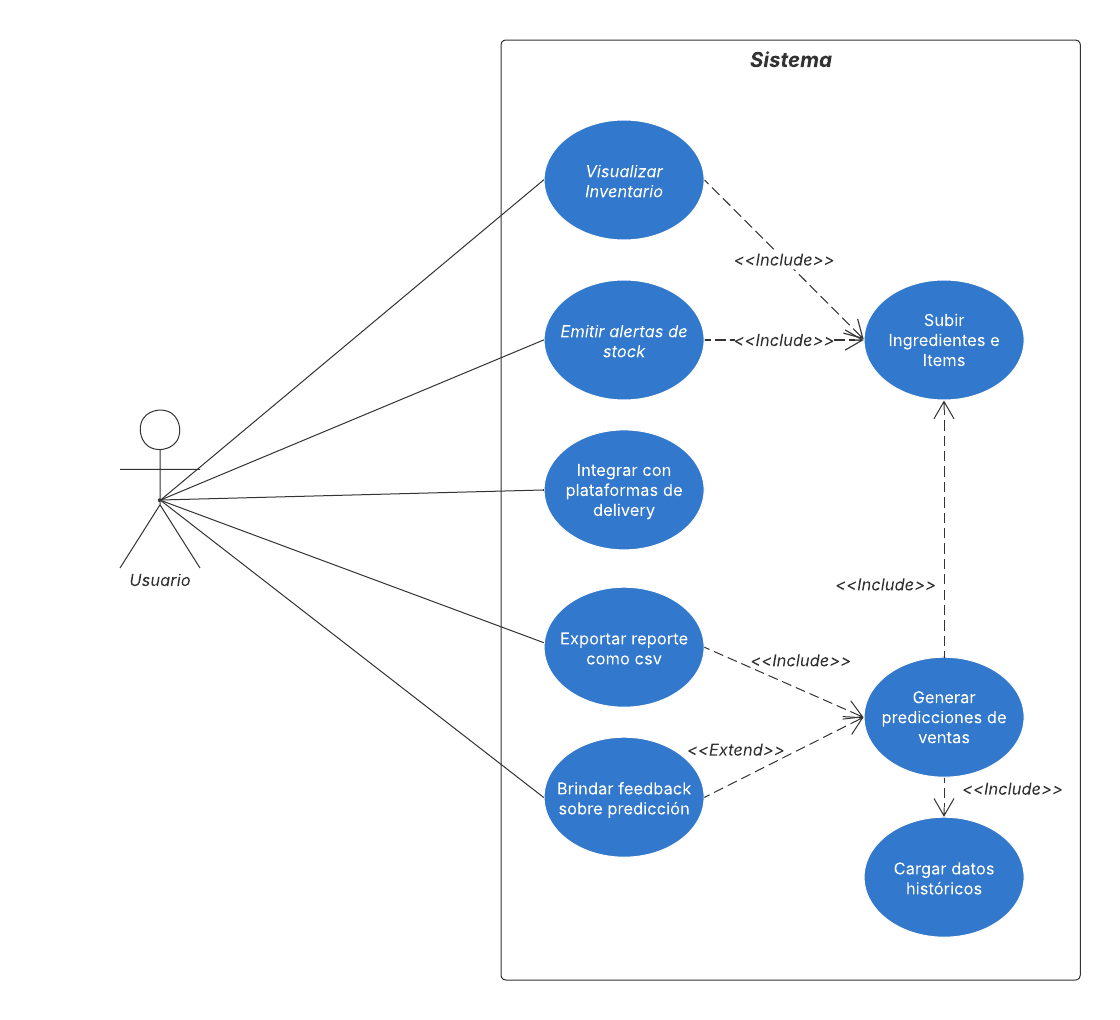
\includegraphics[width=0.7\textwidth]{images/DiagramaCasosDeUsoTesis.png}
    \caption{Diagrama de Casos de Uso}
    \label{fig:casos-de-uso}
\end{figure}

\subsection{Diagramas de Flujo}\label{sec:diagramas-flujo}

Los diagramas de flujo o de procesos son herramientas visuales que representan de manera secuencial los pasos y decisiones que conforman un procedimiento. Su utilización permite clarificar la lógica del negocio, identificar posibles ineficiencias y redundancias, así como facilitar la comunicación entre los equipos técnicos y los usuarios. De esta manera, constituyen un recurso fundamental para comprender, analizar, documentar y mejorar procesos organizacionales \parencite{asq2025flowchart}.

\subsubsection{Registro y Autenticación}

Con el fin de garantizar la seguridad y la personalización de los datos, el acceso a la información y a las funcionalidades críticas de SmartStocker se encuentra restringido a usuarios autenticados. Para ello, la plataforma implementa un flujo de registro inicial y un mecanismo de inicio de sesión que permite identificar de manera única a cada restaurante o local gastronómico.

En la etapa de registro, el usuario debe proporcionar credenciales seguras junto con los datos básicos de su establecimiento. Una vez verificados y almacenados en la base de datos, se habilita la creación de una cuenta que asegura un entorno exclusivo para la gestión de inventario y el análisis de ventas.

\begin{figure}[htbp]
    \centering
    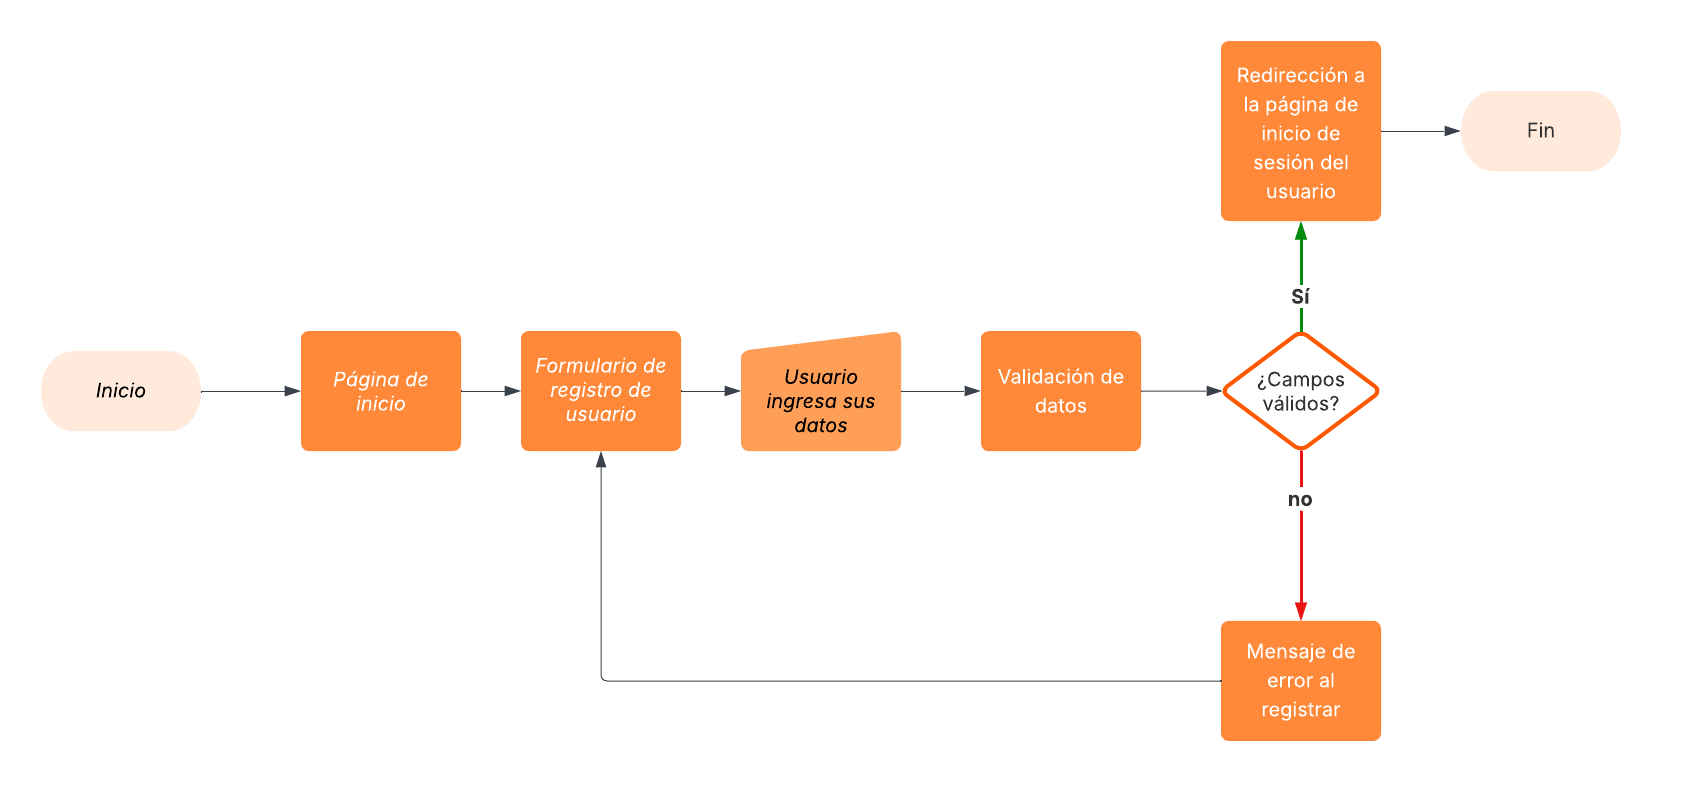
\includegraphics[width=0.7\textwidth]{images/DiagramaRegistroDeUsuario.png}
    \caption{Flujo de Registro del Usuario}
    \label{fig:flujo-registro}
\end{figure}

Posteriormente, mediante la autenticación, los usuarios acceden a su espacio de trabajo personalizado, desde el cual es posible consultar métricas, visualizar predicciones de demanda, administrar productos e ingredientes y recibir alertas relacionadas con el stock disponible. Este proceso de inicio de sesión no solo protege la integridad de la información, sino que también garantiza que las recomendaciones generadas por el sistema respondan a las características particulares de cada negocio gastronómico.

\begin{figure}[htbp]
    \centering
    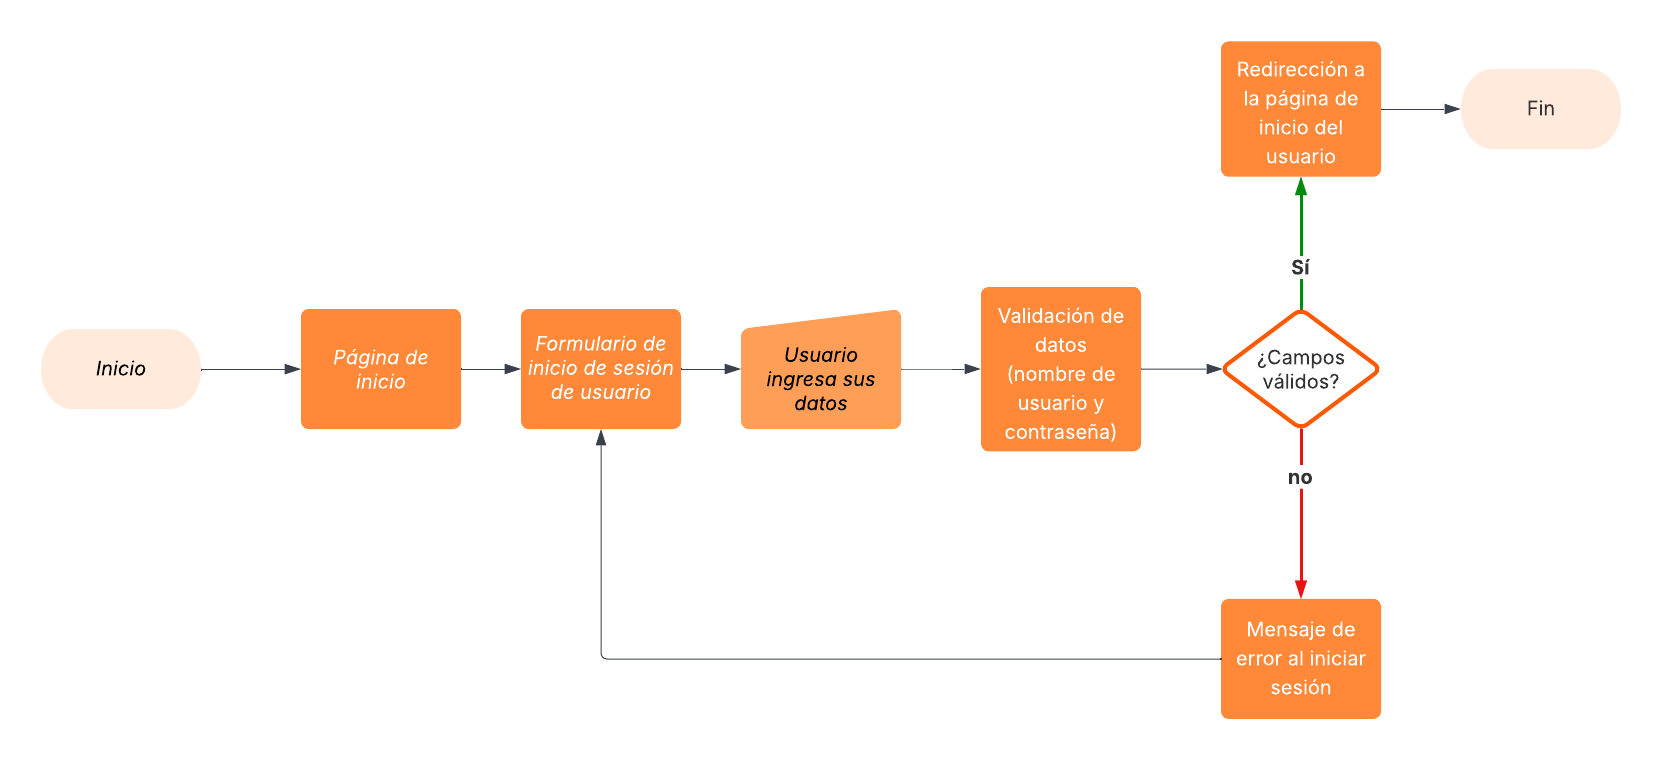
\includegraphics[width=0.7\textwidth]{images/DiagramaInicioDeSesion.png}
    \caption{Flujo de Autenticación del Usuario}
    \label{fig:flujo-autenticacion}
\end{figure}

\subsubsection{Generación de Predicciones}

La capacidad de anticipar la demanda de productos constituye la funcionalidad central de SmartStocker, ya que permite a los restaurantes y locales gastronómicos tomar decisiones fundamentadas sobre compras y reposiciones de insumos. En este proceso, el sistema aplica modelos de Machine Learning que, a partir de datos históricos y variables externas, generan estimaciones confiables de ventas futuras.
\begin{figure}[htbp]
    \centering
    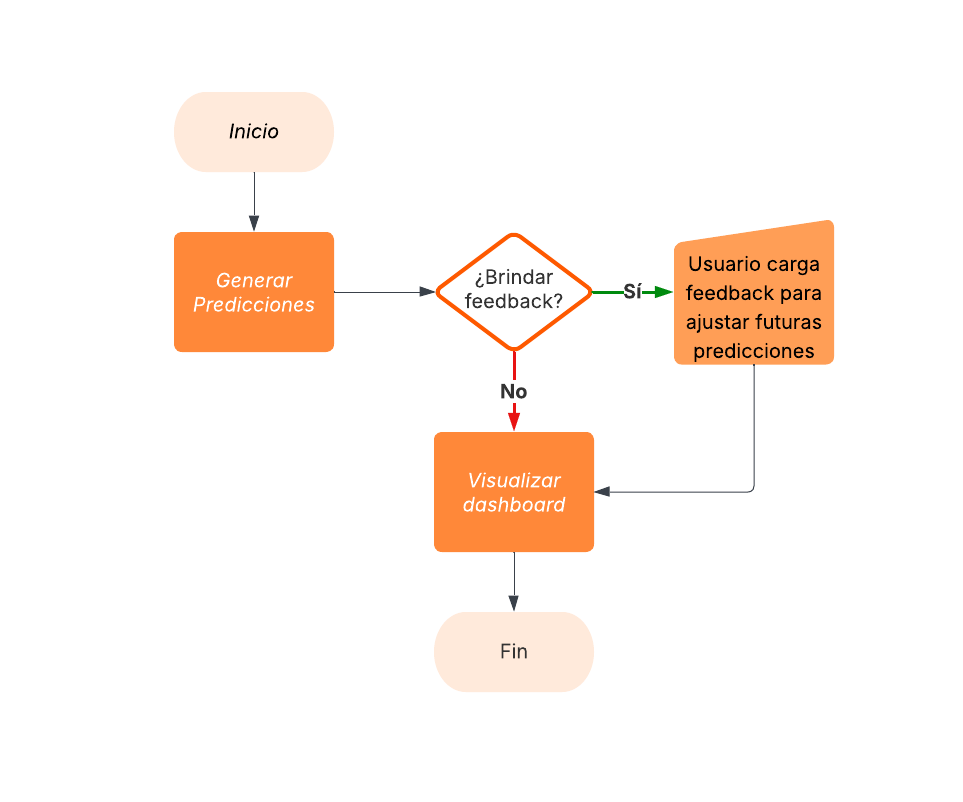
\includegraphics[width=0.7\textwidth]{images/DiagramaDePrediccionTesis.png}
    \caption{Flujo de Predicción de Ventas}
    \label{fig:flujo-prediccion}
\end{figure}

\section{Diseño UX / UI}

El diseño visual de SmartStocker se sustenta en una paleta cromática la cual fue escogida con el propósito de transmitir profesionalismo, confianza y modernidad, atributos que resultan esenciales en un sistema orientado a la toma de decisiones estratégicas en el sector gastronómico. Ahora bien, la elección de los tonos se realizó considerando tanto la dimensión estética como la funcionalidad comunicativa de cada color dentro de la interfaz.

Los colores principales corresponden a una gama de azules, donde el azul corporativo (\#1E40AF) se utiliza en encabezados, botones primarios y elementos de navegación clave. Este tono se asocia tradicionalmente con la seriedad, la estabilidad y la confianza, lo que refuerza la credibilidad del sistema frente a los usuarios que deben basar sus decisiones en datos precisos. Como complemento, el azul claro (\#3B82F6) aparece en estados de interacción como hover y en componentes secundarios, aportando un contraste visual que mantiene la coherencia cromática y facilita la detección rápida de acciones disponibles.

En cuanto a los colores semánticos, se definieron tres que cumplen un rol fundamental en la comunicación de estados del sistema: verde éxito (\#10B981), naranja advertencia (\#F59E0B) y rojo crítico (\#EF4444). Estos colores no solo cumplen con la convención culturalmente reconocida (verde como positivo, rojo como error), sino que también permiten que el usuario identifique de forma inmediata la condición de un insumo o la validez de una acción.

Los colores de apoyo, grises en diferentes intensidades y blanco como fondo principal, cumplen la función de dar equilibrio visual. El gris oscuro (\#1F2937) se emplea en textos principales para asegurar legibilidad, mientras que el gris medio (\#6B7280) se reserva para información secundaria, evitando así la sobrecarga cognitiva. Además, el gris claro (\#F3F4F6) y el azul muy claro (\#EFF6FF) sirven como fondos sutiles y separadores, permitiendo estructurar la información en bloques diferenciados sin necesidad de líneas divisorias excesivas.

En conjunto, esta paleta de colores no responde únicamente a una intención estética, sino que está al servicio de la usabilidad, la accesibilidad y la experiencia de usuario. Cada tonalidad se integra en un sistema visual coherente que facilita la navegación, refuerza el reconocimiento de patrones y garantiza que los usuarios puedan interactuar con la plataforma de forma intuitiva y eficiente.

\begin{table}[htbp]
    \centering
    \begin{tabular}{|l|c|c|}
        \hline
        \textbf{Categoría} & \textbf{Color} & \textbf{Código Hex} \\ \hline
        Azul corporativo & \cellcolor[HTML]{1E40AF} & \#1E40AF \\ \hline
        Azul claro & \cellcolor[HTML]{3B82F6} & \#3B82F6 \\ \hline
        Verde éxito & \cellcolor[HTML]{10B981} & \#10B981 \\ \hline
        Naranja advertencia & \cellcolor[HTML]{F59E0B} & \#F59E0B \\ \hline
        Rojo crítico & \cellcolor[HTML]{EF4444} & \#EF4444 \\ \hline
        Gris oscuro (texto principal) & \cellcolor[HTML]{1F2937} & \#1F2937 \\ \hline
        Gris medio (texto secundario) & \cellcolor[HTML]{6B7280} & \#6B7280 \\ \hline
        Gris claro (fondos) & \cellcolor[HTML]{F3F4F6} & \#F3F4F6 \\ \hline
        Azul muy claro (fondos) & \cellcolor[HTML]{EFF6FF} & \#EFF6FF \\ \hline
    \end{tabular}
    \caption{Paleta de colores empleada en SmartStocker}
    \label{tab:paleta-colores}
\end{table}

\section{Pantallas de la aplicación}

A continuación, se presentan las principales pantallas de la aplicación SmartStocker, organizadas según el flujo de interacción del usuario. Estas capturas ilustran tanto la experiencia inicial (landing e inicio de sesión) como la gestión de datos (ingredientes, ítems) y las funcionalidades clave de predicción de ventas.

\begin{figure}[htbp]
    \centering
    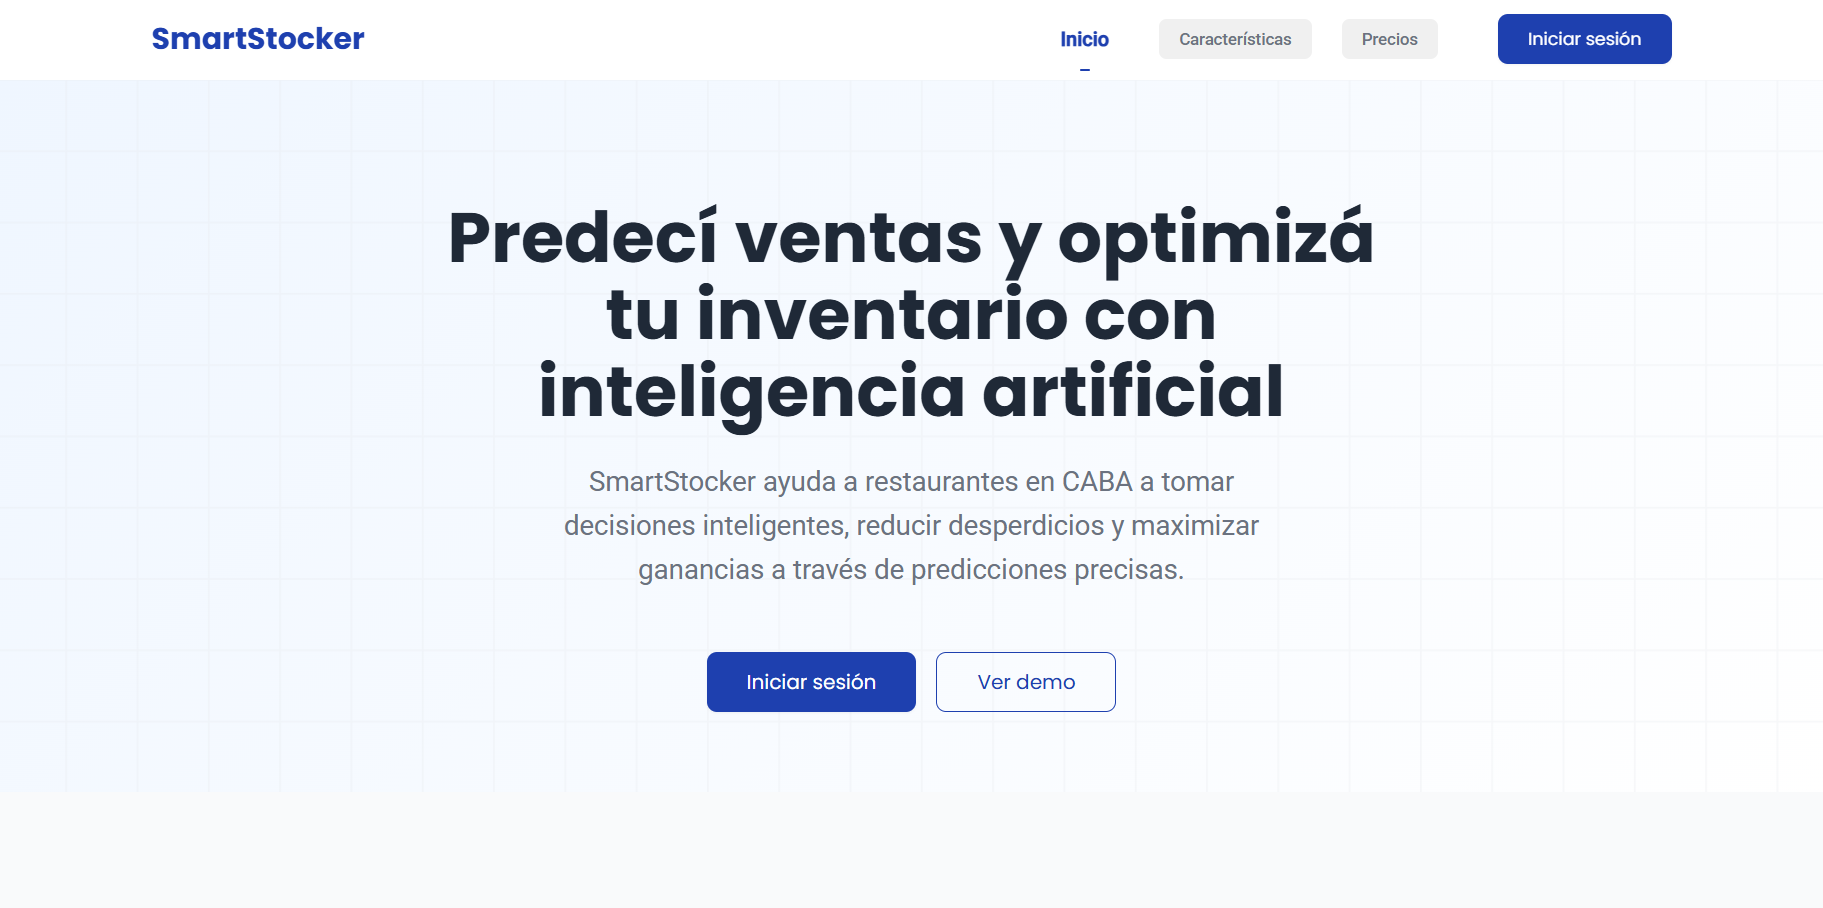
\includegraphics[width=0.9\textwidth]{images/landing1.png}
    \caption{Pantalla de inicio (Landing) – Parte 1}
    \label{fig:ux-landing1}
\end{figure}

\begin{figure}[htbp]
    \centering
    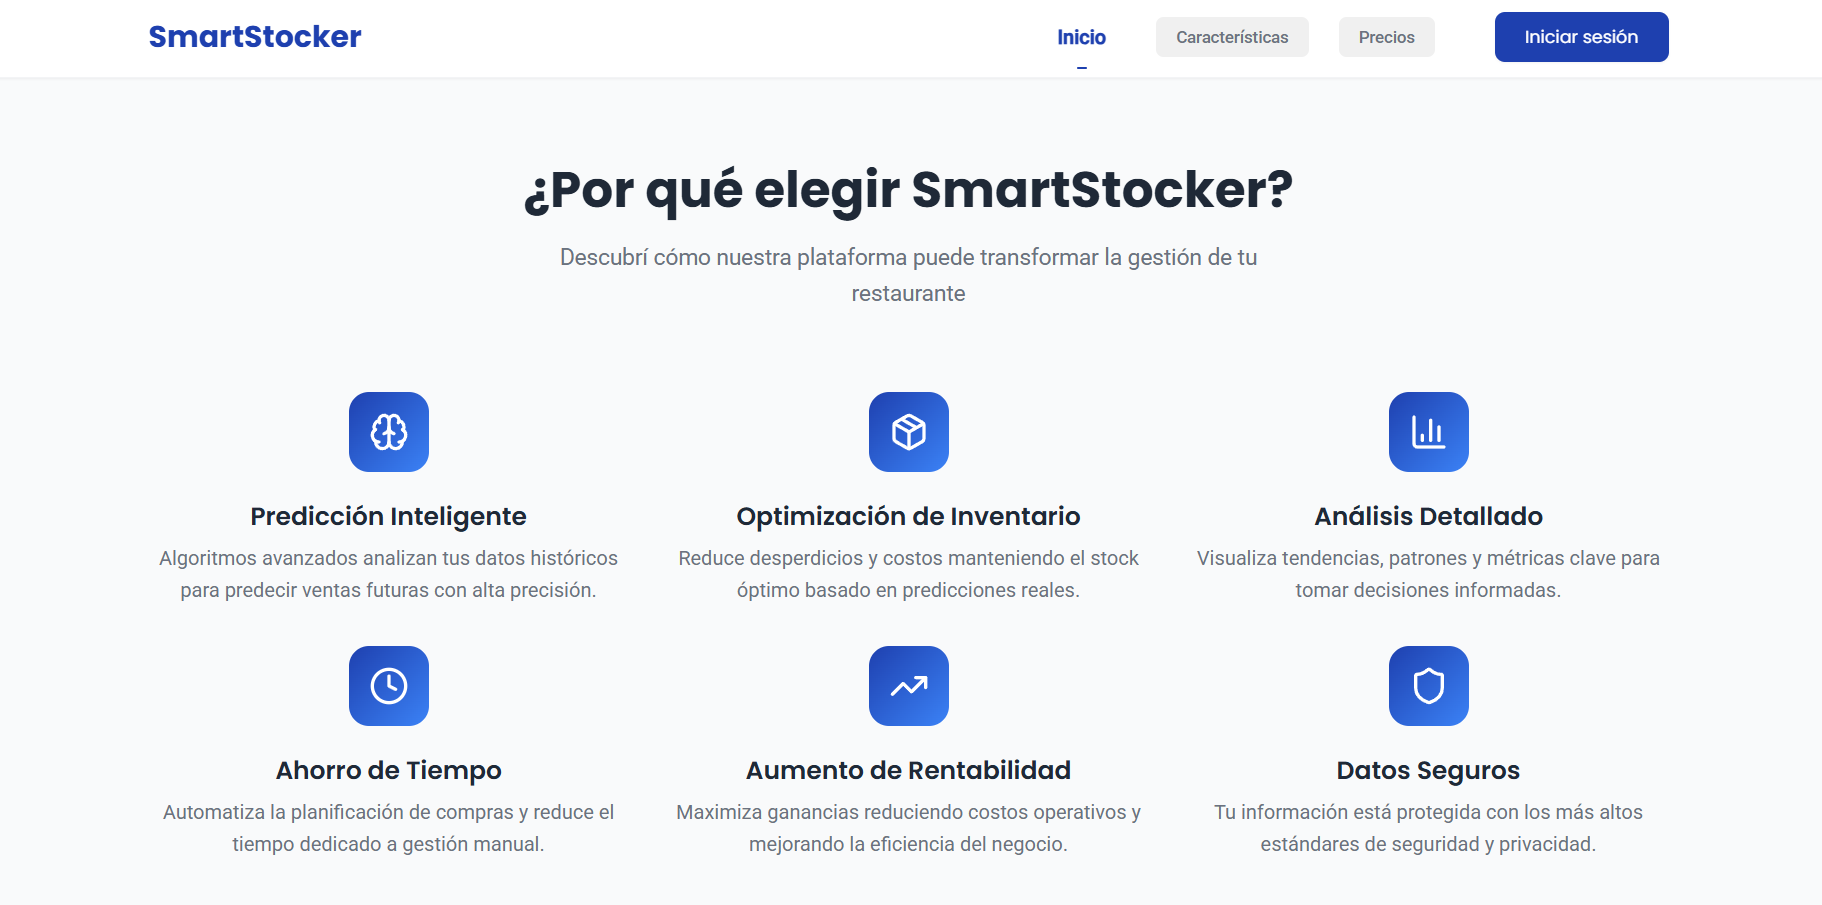
\includegraphics[width=0.9\textwidth]{images/landing2.png}
    \caption{Pantalla de inicio (Landing) – Parte 2}
    \label{fig:ux-landing2}
\end{figure}

\begin{figure}[htbp]
    \centering
    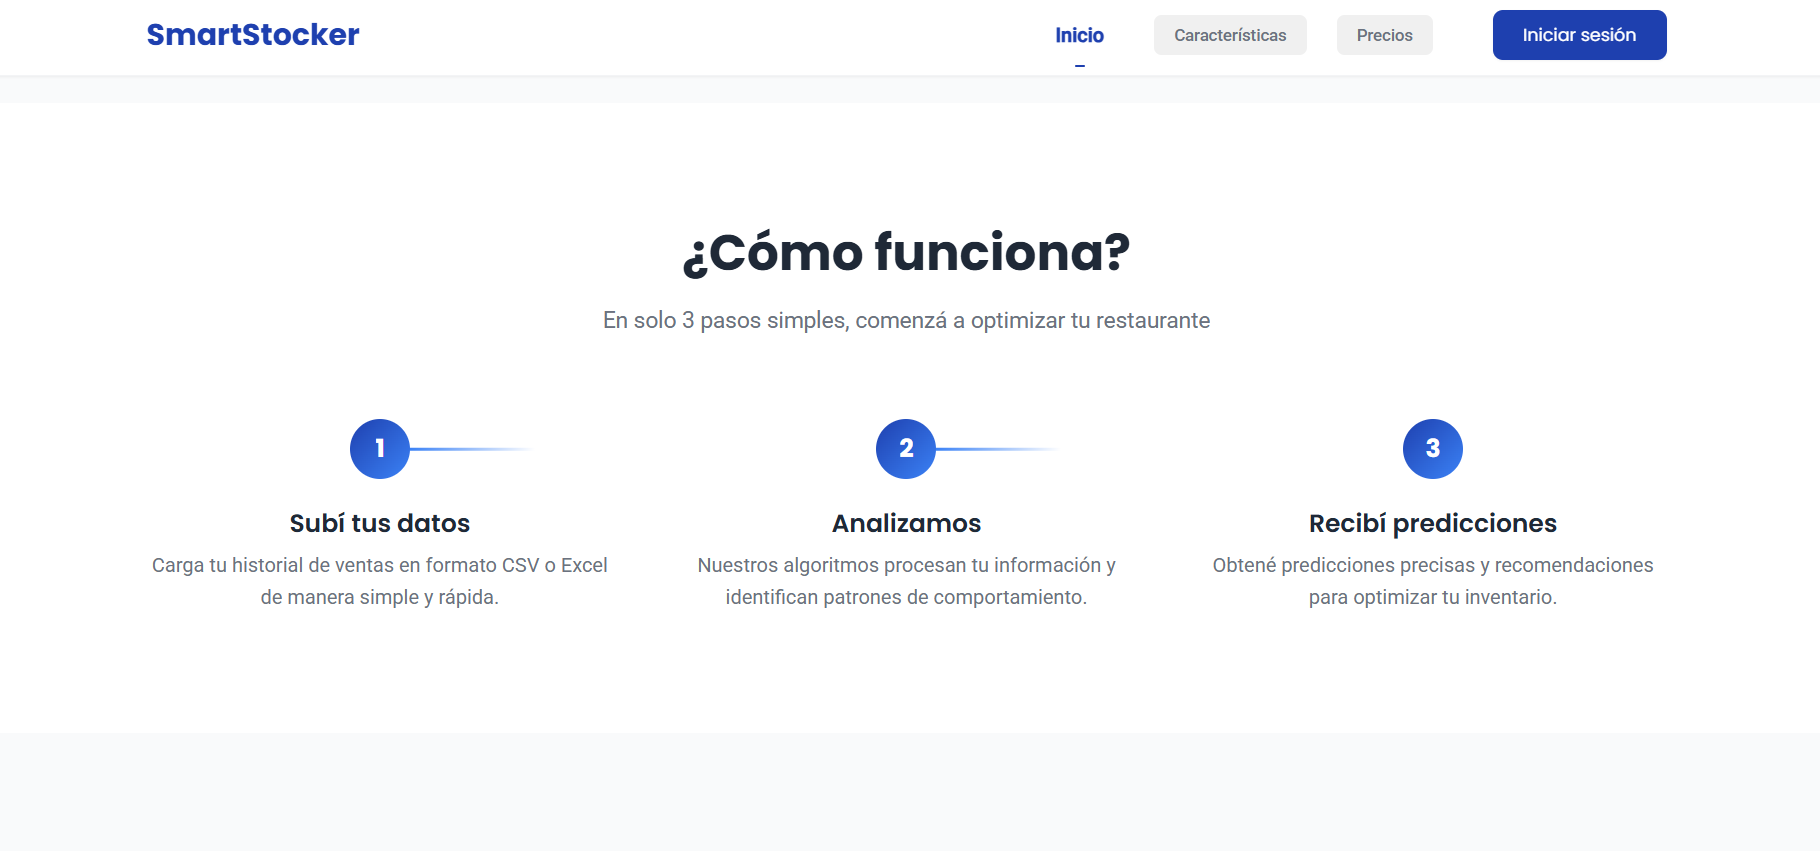
\includegraphics[width=0.9\textwidth]{images/landing3.png}
    \caption{Pantalla de inicio (Landing) – Parte 3}
    \label{fig:ux-landing3}
\end{figure}

\begin{figure}[htbp]
    \centering
    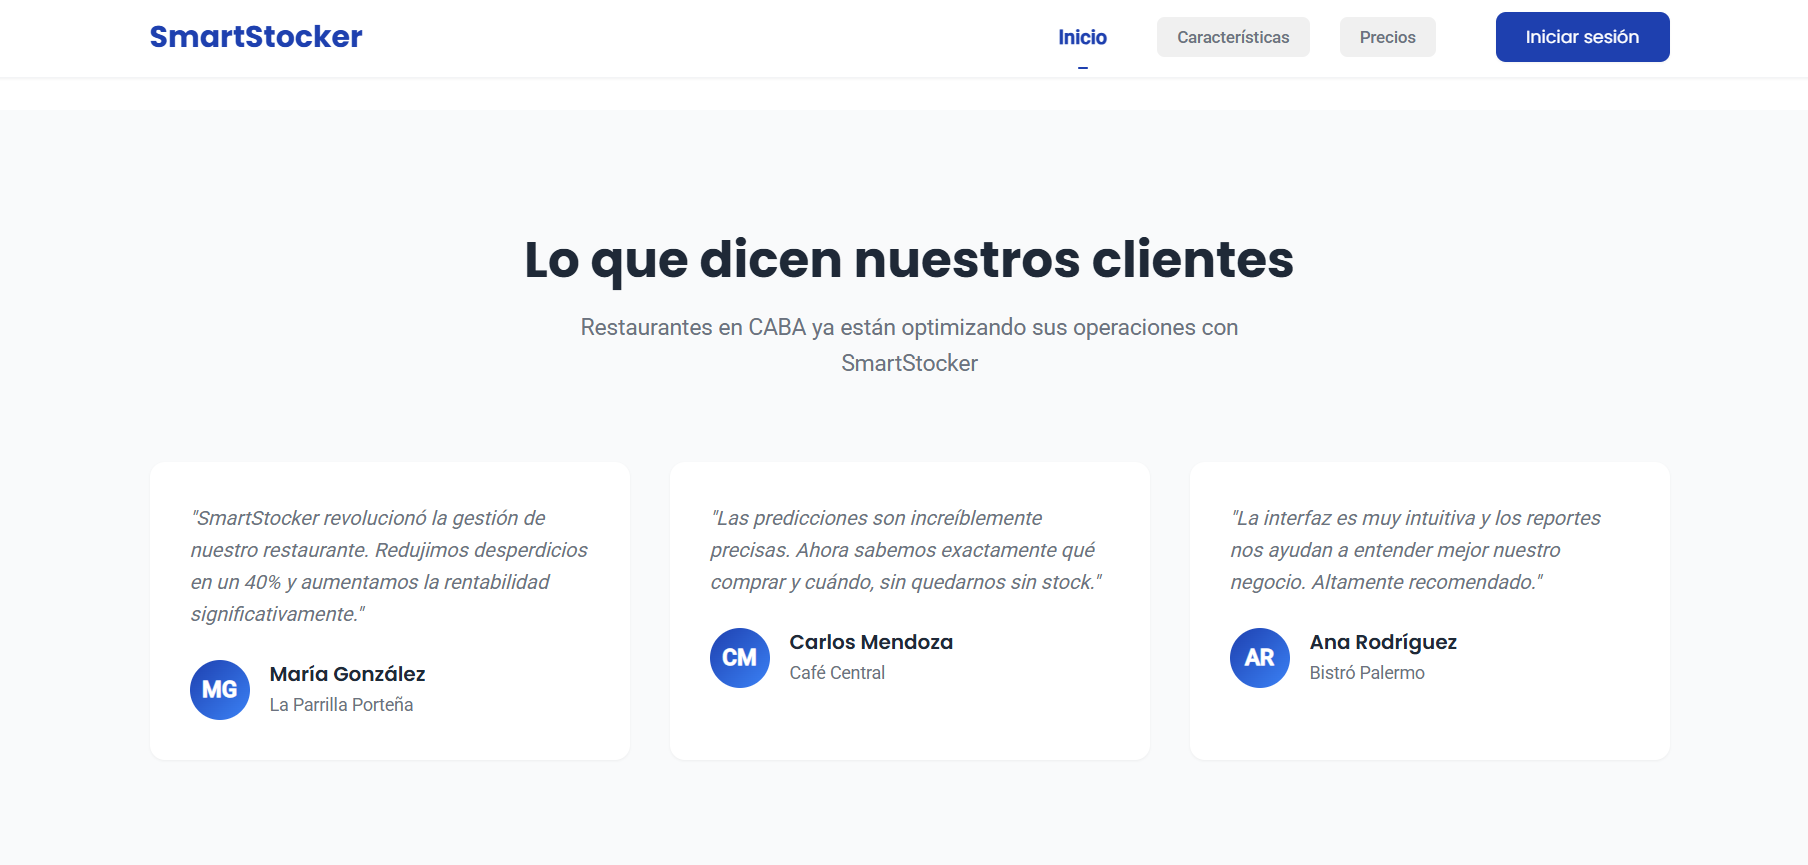
\includegraphics[width=0.9\textwidth]{images/landing4.png}
    \caption{Pantalla de inicio (Landing) – Parte 4}
    \label{fig:ux-landing4}
\end{figure}

\begin{figure}[htbp]
    \centering
    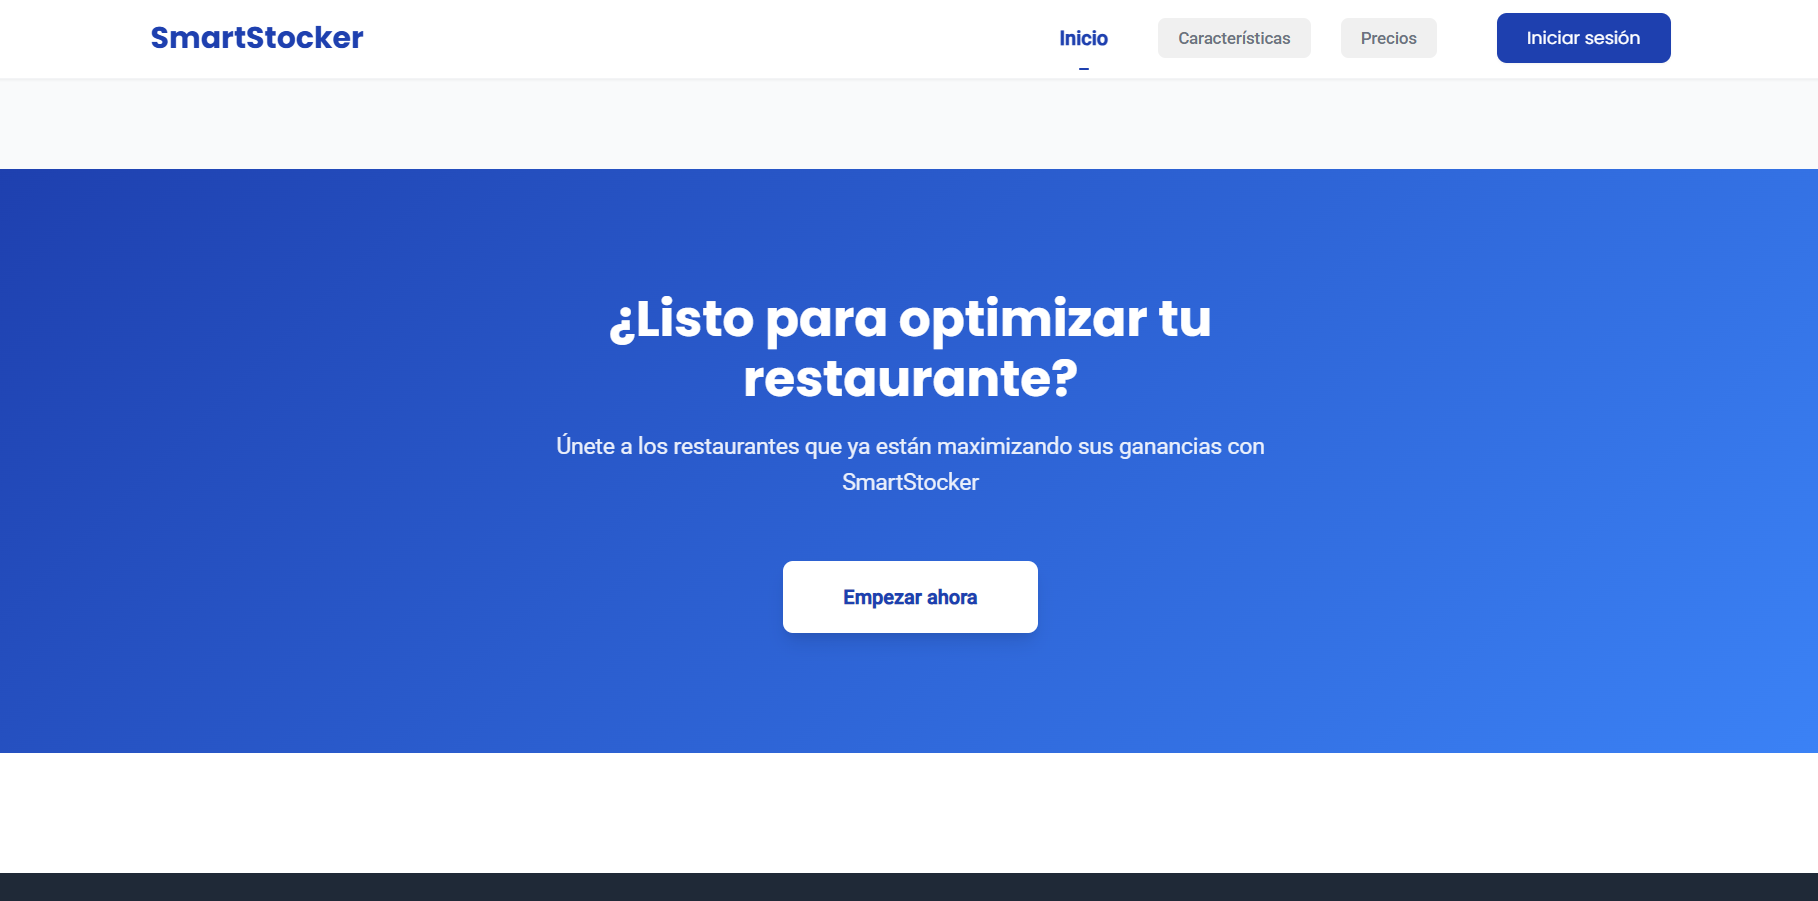
\includegraphics[width=0.9\textwidth]{images/landing5.png}
    \caption{Pantalla de inicio (Landing) – Parte 5}
    \label{fig:ux-landing5}
\end{figure}

\begin{figure}[htbp]
    \centering
    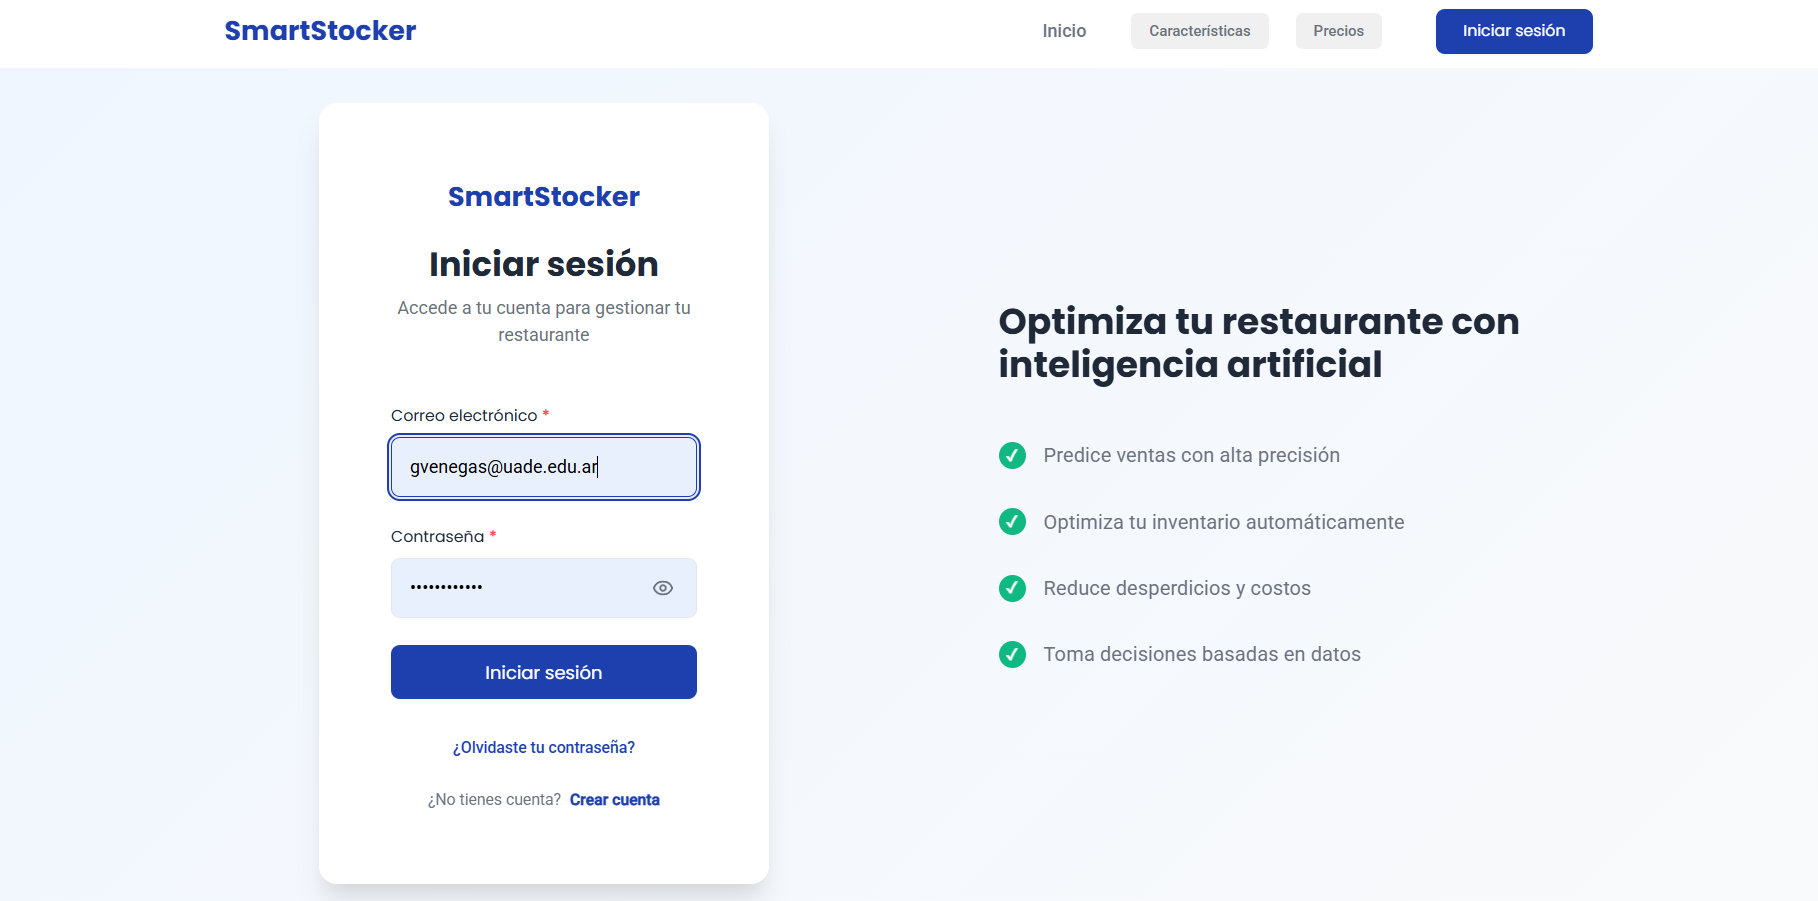
\includegraphics[width=0.9\textwidth]{images/login.png}
    \caption{Pantalla de inicio de sesión}
    \label{fig:ux-login}
\end{figure}

\begin{figure}[htbp]
    \centering
    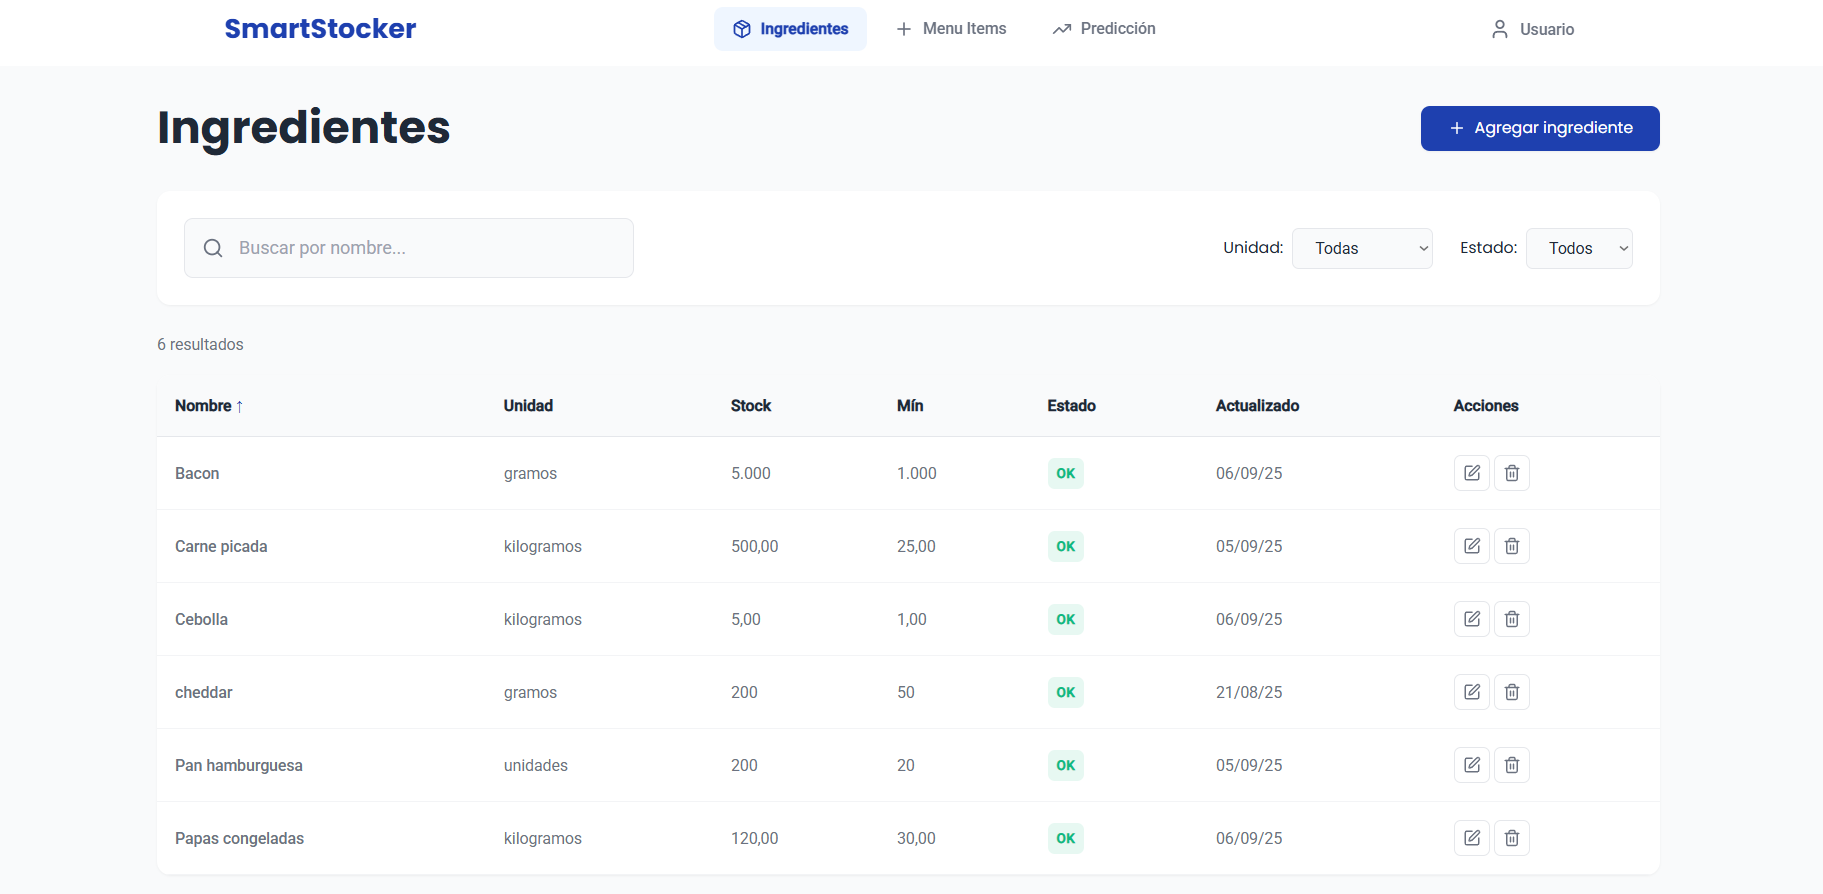
\includegraphics[width=0.9\textwidth]{images/ingredientes.png}
    \caption{Pantalla de gestión de ingredientes}
    \label{fig:ux-ingredientes}
\end{figure}

\begin{figure}[htbp]
    \centering
    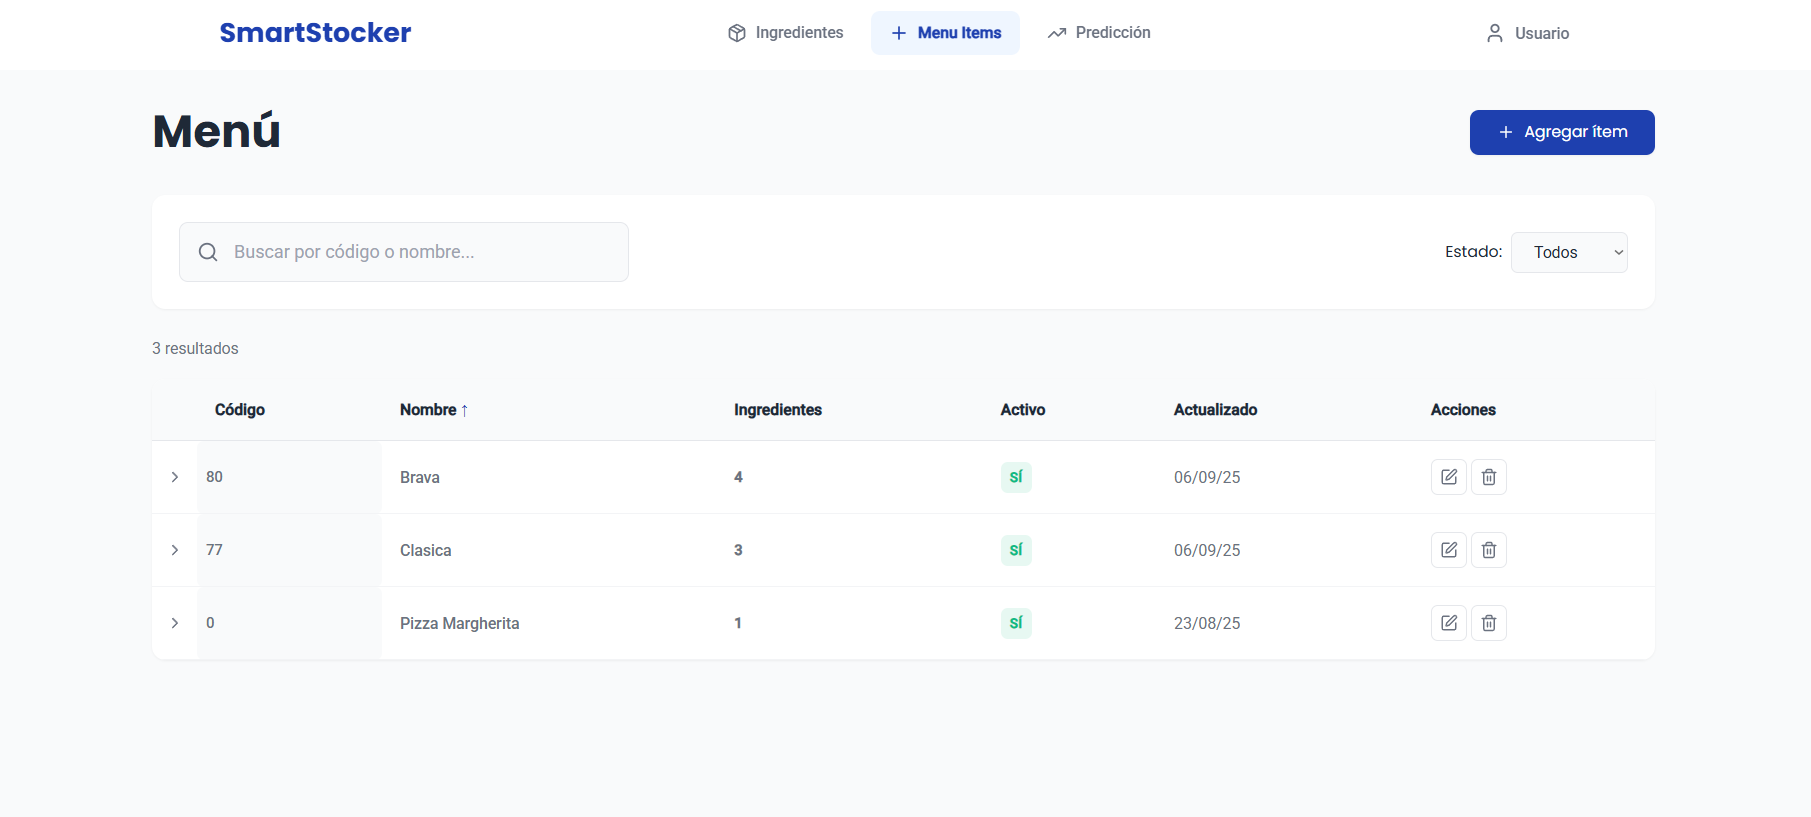
\includegraphics[width=0.9\textwidth]{images/items.png}
    \caption{Pantalla de gestión de ítems}
    \label{fig:ux-items}
\end{figure}

\begin{figure}[htbp]
    \centering
    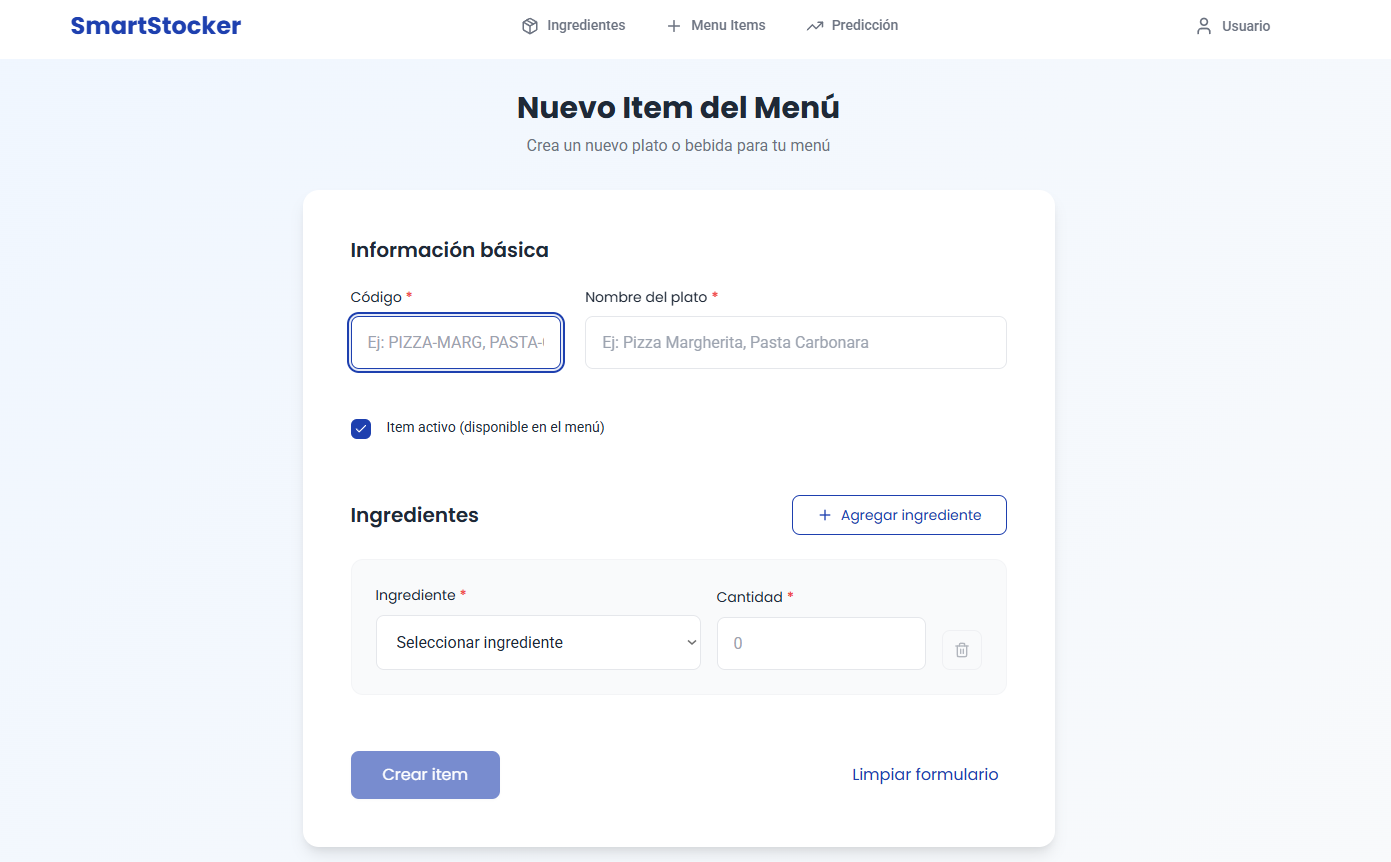
\includegraphics[width=0.9\textwidth]{images/nuevoItem.png}
    \caption{Pantalla para agregar un nuevo ítem}
    \label{fig:ux-nuevo-item}
\end{figure}

\begin{figure}[htbp]
    \centering
    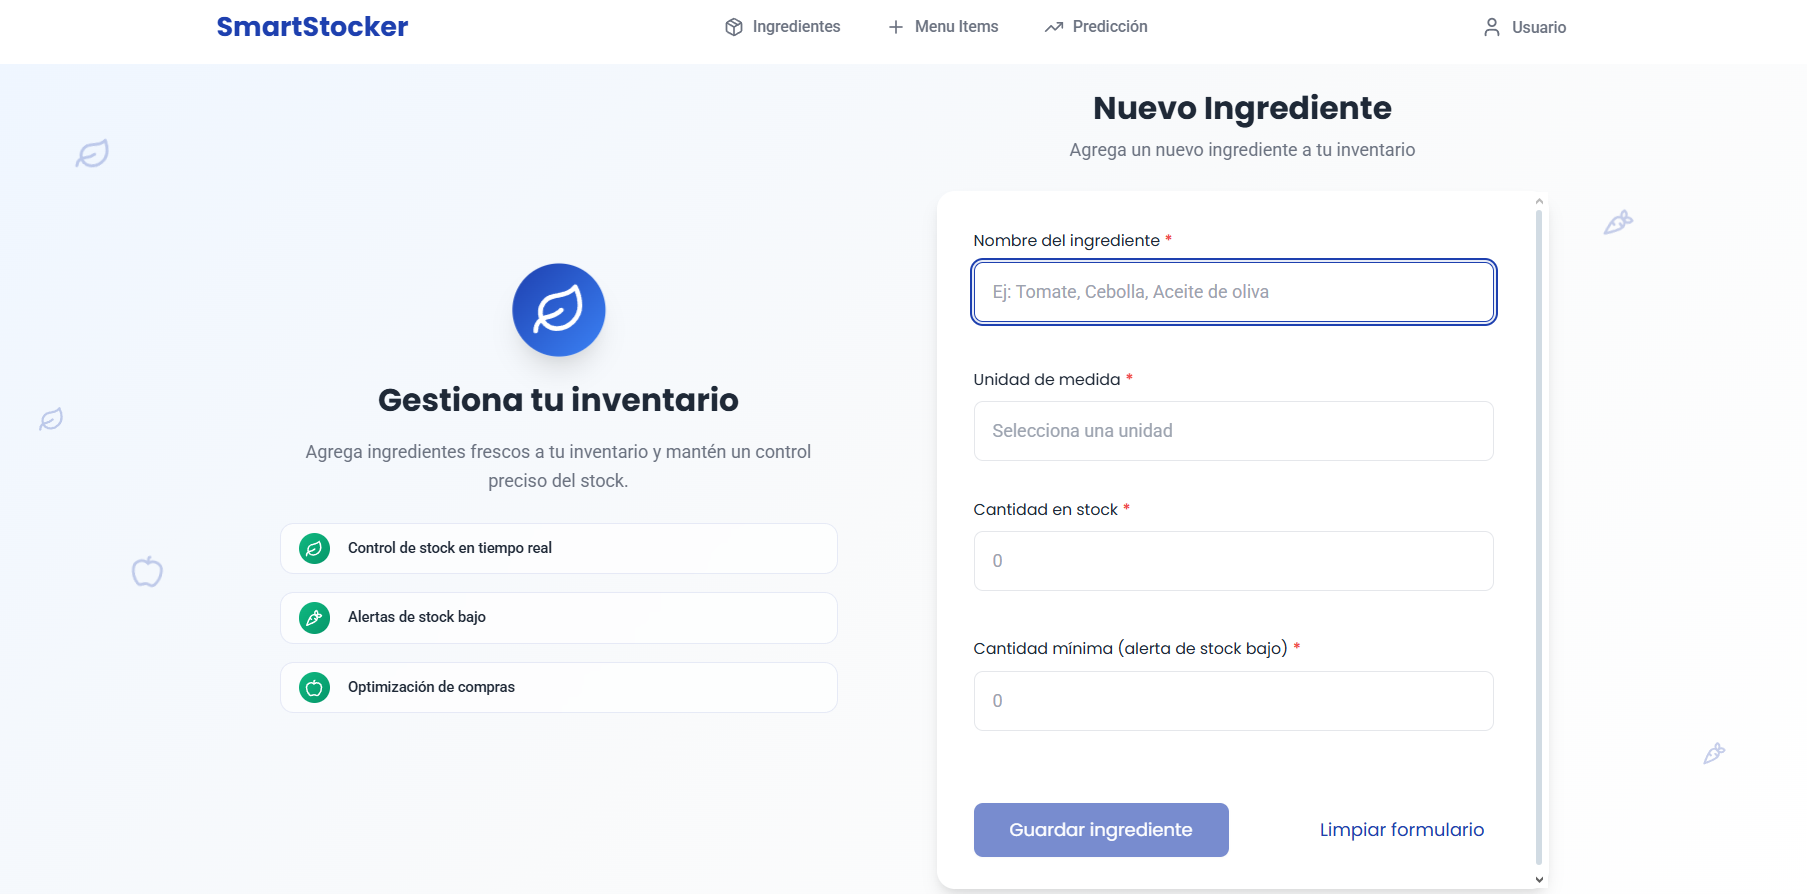
\includegraphics[width=0.9\textwidth]{images/nuevoIngrediente.png}
    \caption{Pantalla para agregar un nuevo ingrediente}
    \label{fig:ux-nuevo-ingrediente}
\end{figure}

\begin{figure}[htbp]
    \centering
    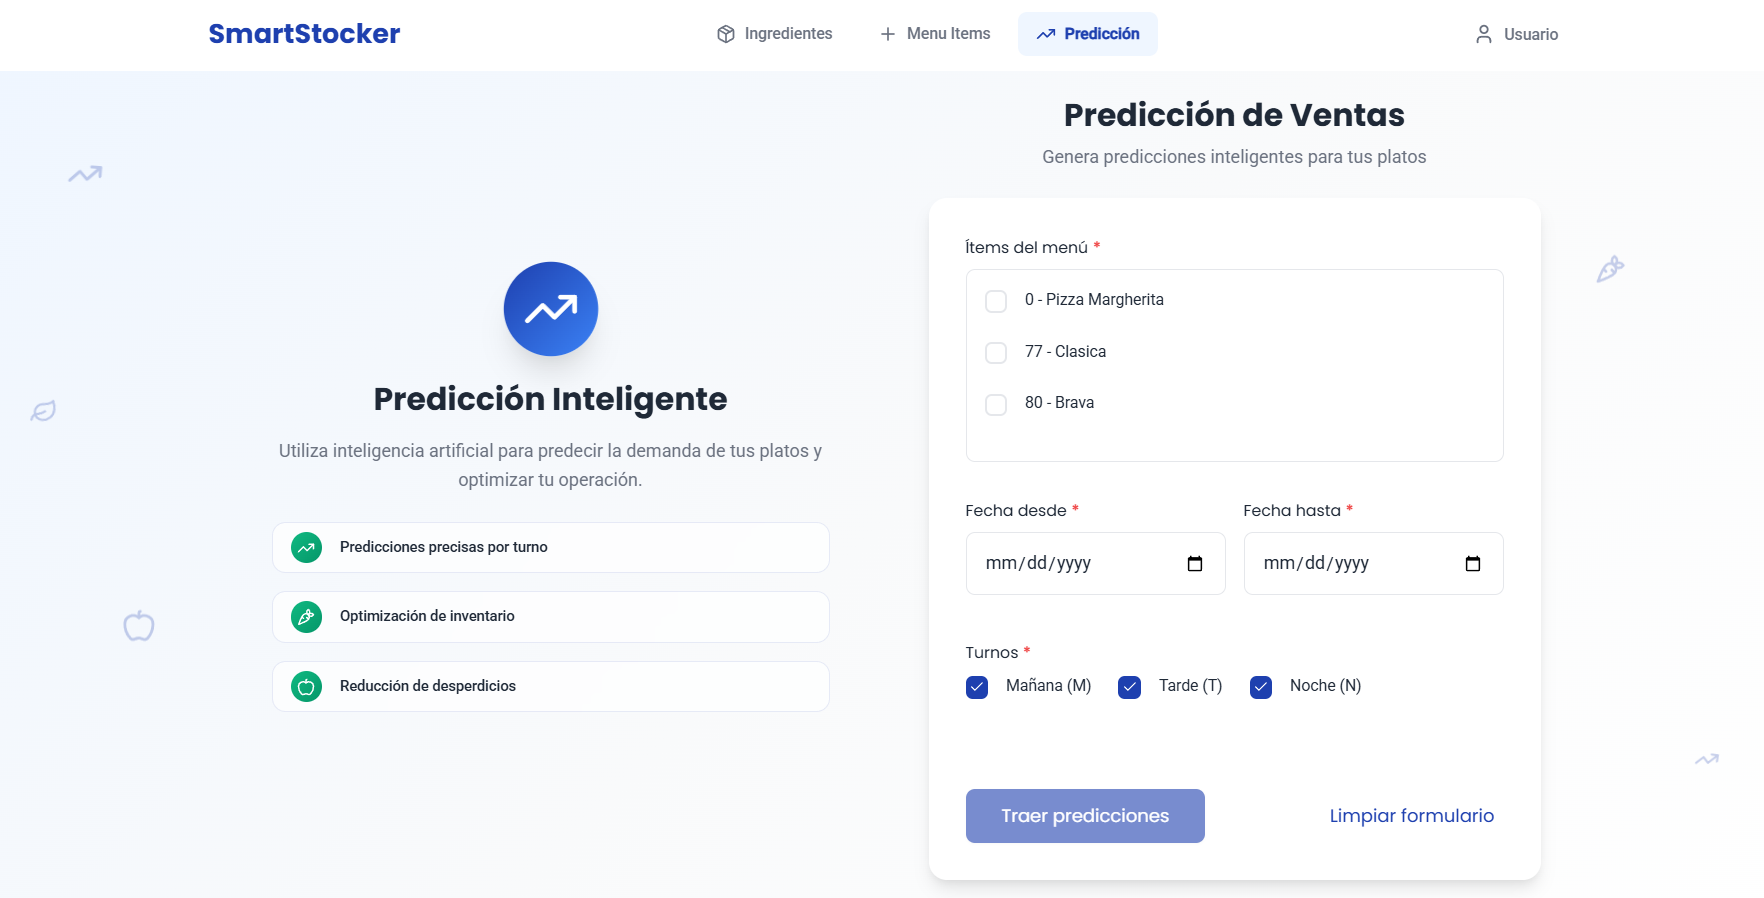
\includegraphics[width=0.9\textwidth]{images/predicciones.png}
    \caption{Pantalla consolidada de predicciones}
    \label{fig:ux-predicciones}
\end{figure}

\begin{figure}[htbp]
    \centering
    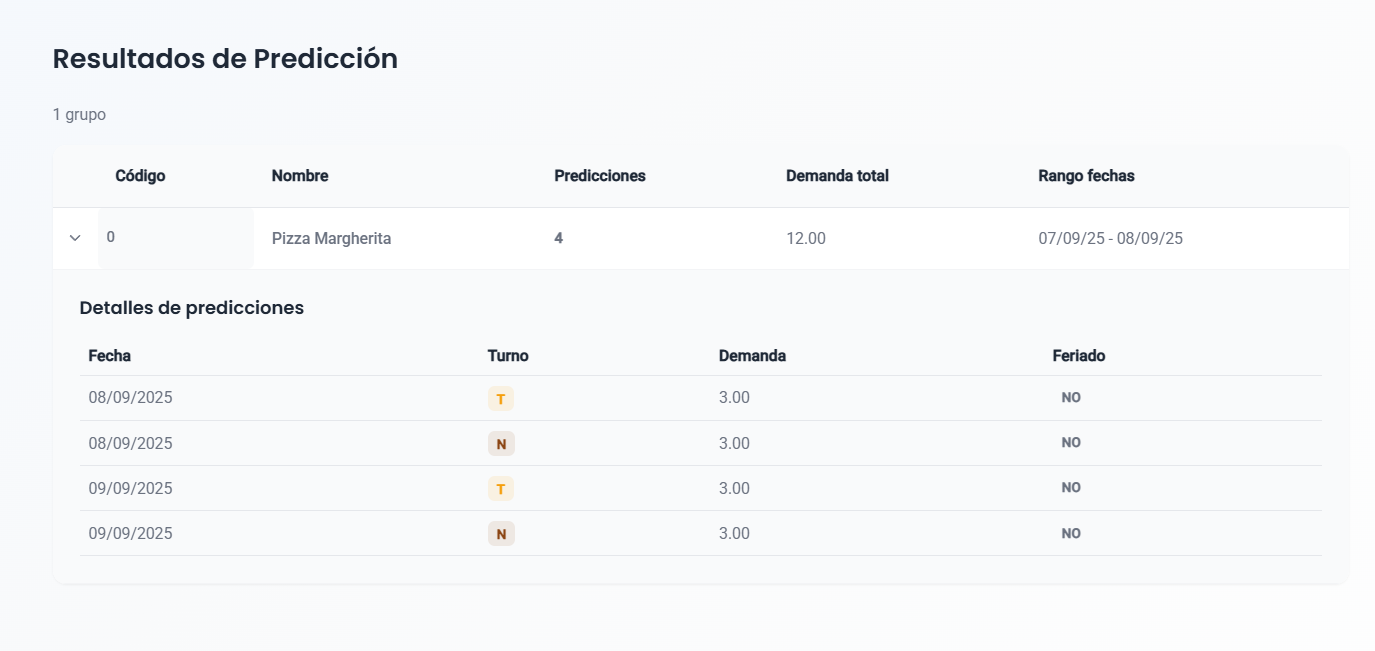
\includegraphics[width=0.9\textwidth]{images/prediccion1.png}
    \caption{Resultado de predicciones}
    \label{fig:ux-prediccion1}
\end{figure}

\begin{figure}[htbp]
    \centering
    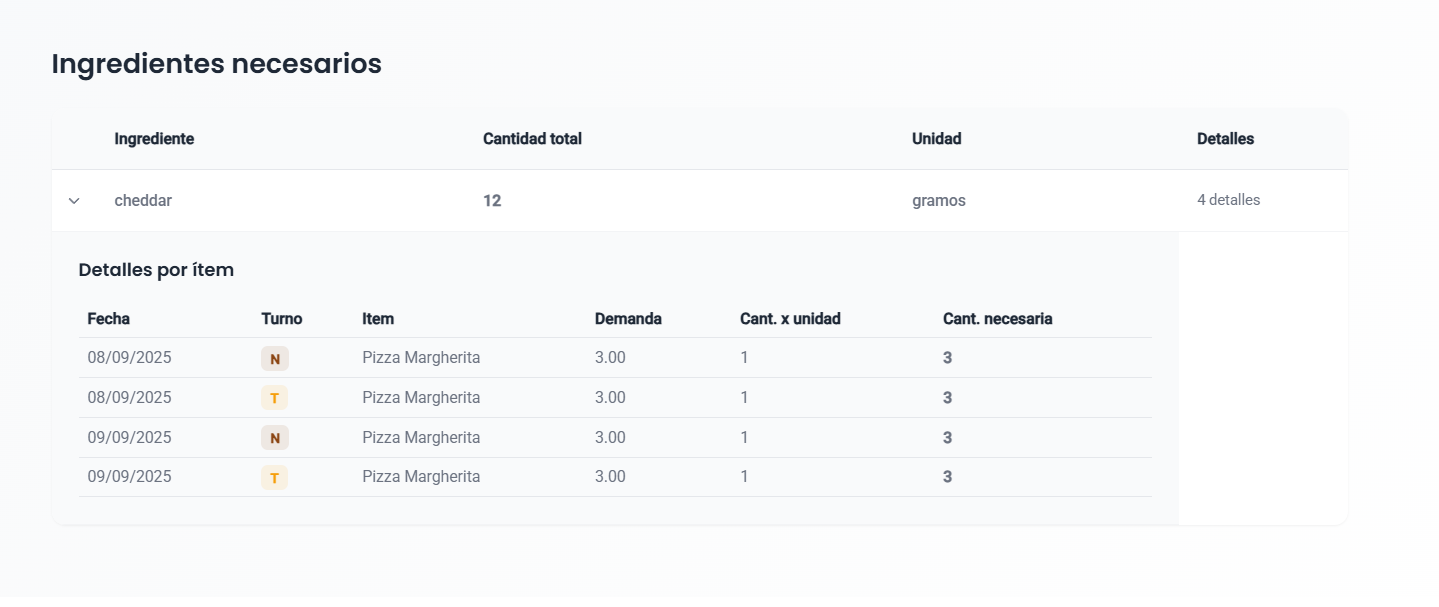
\includegraphics[width=0.9\textwidth]{images/prediccion2.png}
    \caption{Ingredientes necesarios}
    \label{fig:ux-prediccion2}
\end{figure}

\section{Funcionalidades}\label{sec:funcionalidades}

\subsection{Predicción de Ventas}\label{sec:prediccion-ventas}

En el sector gastronómico, la capacidad de anticipar la demanda se ha convertido en un factor estratégico para reducir pérdidas, optimizar el uso de insumos y garantizar la continuidad del servicio. Bajo dicha premisa, SmartStocker incorpora un módulo de predicciones como una de sus funcionalidades principales. El sistema aplica técnicas de aprendizaje automático que permiten transformar datos históricos y registros actuales en estimaciones de ventas futuras. 

El objetivo de esta funcionalidad es reemplazar las decisiones basadas únicamente en la experiencia o la intuición por un enfoque sistemático apoyado en datos, incrementando la objetividad en la gestión del inventario. Además, su integración con fuentes externas de información le otorga la capacidad de adaptarse a contextos cambiantes, como la estacionalidad, los feriados o incluso factores climáticos que pueden influir en el consumo.

\subsection{Fuentes de Datos}\label{sec:fuentes-datos}

El modelo predictivo requiere datos de calidad para generar resultados confiables. Con este fin, la plataforma web admite dos vías principales de recopilación:

\begin{itemize}
    \item \textbf{Carga manual de datos mediante archivos CSV}: esta modalidad permite a los locales gastronómicos incorporar sus registros históricos directamente desde sistemas internos o planillas de control. Para este fin, se determinó que el formato esperado para archivos CSV es:
    \begin{itemize}
        \item Fecha venta: dd/mm/aaaa hh:mm:ss
        \item Producto: con el mismo nombre usado al generar el producto en la aplicación.
        \item Cantidad.
    \end{itemize}

    \item \textbf{Integración automática con sistemas de venta}: este mecanismo posibilita la importación continua de pedidos en tiempo real desde aplicaciones como PedidosYa. Con ello, el sistema asegura la actualización permanente del conjunto de datos, reduciendo la dependencia exclusiva de registros históricos y adaptándose a la dinámica diaria del negocio.
\end{itemize}

\subsection{Gestion de ingredientes e items del menu}\label{sec:carga-datos}

Para que el sistema pueda calcular el inventario sugerido, es necesario que el usuario cargue los ingredientes que utiliza en su local y los vincule con los productos gastronómicos que ofrece en su menú. Esta funcionalidad permite al usuario definir y administrar tanto los ingredientes como los items del menu, permitiendo, en el caso particular de los ingredientes, realizar esta carga no solo desde la UI, sino tambien de forma masiva a traves de un archivo, a fin de simplificar la operatoria en caso de que el usuario cuente con un listado extenso.

\subsection{Procesamiento Predictivo}\label{sec:procesamiento-predictivo}

El procesamiento predictivo constituye el núcleo técnico de la funcionalidad de SmartStocker. Una vez recopilados los datos históricos y actuales, el sistema los somete a un proceso de depuración y normalización que asegura la consistencia y homogeneidad de los registros. Este preprocesamiento incluye la eliminación de valores atípicos, la imputación de datos faltantes y la transformación de variables temporales (como la estacionalidad o los turnos horarios) en características relevantes para el modelo.

Posteriormente, los datos son utilizados para entrenar algoritmos de aprendizaje supervisado, dentro de los cuales se evaluaron diferentes enfoques, priorizando modelos de regresión y técnicas de boosting como CatBoost, debido a su robustez en contextos con variables categóricas y a su capacidad de reducir el sobreajuste. Estos modelos generan proyecciones de ventas futuras en base a patrones identificados, incorporando tanto las tendencias históricas como variables externas tales como clima, feriados y días de la semana.

Las predicciones se ejecutan bajo demanda, es decir, cada vez que el usuario lo requiera dentro de la plataforma, lo que garantiza resultados actualizados y adaptados al contexto puntual de planificación del negocio, integrando un mecanismo de retroalimentación continua (feedback loop) mediante el cual los usuarios validan si las estimaciones reflejaron la demanda real observada; esa información se reintegra al modelo para ajustar progresivamente su precisión, personalizando las predicciones al contexto específico de cada restaurante y favoreciendo la evolución de SmartStocker ante escenarios cambiantes.

En consecuencia, el procesamiento predictivo de SmartStocker no se limita a entregar un valor numérico de ventas estimadas, sino que constituye un sistema adaptable y evolutivo, orientado a respaldar la toma de decisiones estratégicas en la gestión de inventarios gastronómicos.

\subsection{Cálculo de Inventario Sugerido}\label{sec:calculo-inventario}

Una vez obtenidas las predicciones de ventas, los resultados obtenidos son vinculados con la lista de ingredientes definida por el restaurante. De esta manera, se genera un cálculo automático del inventario recomendado, minimizando tanto los riesgos de desabastecimiento como los costos derivados de un exceso de stock. 

\subsection{Notificación de Alertas}\label{sec:alertas}

El módulo de notificaciones cumple un rol preventivo. Cada vez que un insumo alcanza un nivel inferior al umbral configurado por el usuario, el sistema genera una alerta en el tablero principal y, en futuras versiones, podrá enviarlas vía correo electrónico o notificaciones push.

El valor de este componente radica en su capacidad para evitar interrupciones operativas. En un negocio gastronómico, la ausencia de un ingrediente clave no solo afecta la venta de un plato específico, sino que también impacta en la experiencia del cliente y en la reputación del local. Por esta razón, las alertas de stock bajo no deben considerarse únicamente como un aviso técnico, sino como un mecanismo de aseguramiento de la calidad del servicio.


\section{Arquitectura de la solución}\label{sec:arquitectura-solucion}
En esta sección se presenta la arquitectura de SmartStocker, detallando las tecnologías empleadas para su diseño técnico y funcional. La arquitectura funciona como marco conceptual que sustenta cada componente del sistema y especifica las interacciones y dependencias entre las distintas partes que lo componen.

\subsection{Diagrama de Arquitectura conceptual}\label{sec:arquitectura-conceptual}
En relación con la arquitectura de alto nivel de SmartStocker, se propone un modelo de tres capas que organiza la solución, asegurando una separación clara de responsabilidades y mejorando la escalabilidad. Esta estructura está diseñada para optimizar tanto la interacción con el usuario como el procesamiento y almacenamiento de los registros de venta y los resultados de inferencia generados por los modelos predictivos.

La primera capa —Capa de Presentación (Presentation Layer)— agrupa la interfaz y la experiencia de usuario. En ella se implementa el frontend de SmartStocker con Next.js y se despliega mediante AWS Amplify, aprovechando sus capacidades de hosting y CI/CD. Esta capa permite a los usuarios interactuar con la plataforma, gestionar sus productos e ingredientes, visualizar recomendaciones y alertas, y realizar operaciones de predicciones de venta de forma responsiva y orientada a la operativa diaria.

La Capa de Negocio (Business Layer) constituye el núcleo lógico de SmartStocker y se organiza en tres componentes principales. El primero es una API REST que actúa como puente entre la capa de presentación y los servicios backend; a través de ella se gestionan las sesiones y la autorización, se exponen los endpoints para solicitar predicciones y gestionar productos, ingredientes, y alertas, y se que incluye la lógica necesaria para atender las demandas de la interfaz de usuario de forma segura y consistente. Esta se encuentra desarollada con Node.js, a fin de aprovechar lo mas posible su integracion nativa con Next.js, y la simpleza a la hora de desplegar la api de forma serverless mediante AWS Lambda. El segundo es el pipeline de ETL, encargado de recibir los datos de ventas en tiempo real desde los sistemas externos, procesarlos, enriquecerlos, y dejarlos listos para ser usados por el modelo. Por último, el pipeline de ML será el encargado de realizar el entrenamiento del modelo, ya sea de forma periódica u on demand, y de dejarlo disponible para su uso en las operaciones de inferencia. La logica de ambos pipelines se encuentra desarollada en Python, a fin de aprovechar las distintas librerías y frameworks disponibles para el procesamiento de datos y machine learning, y se encuentran implementados mediante AWS Lambda.

Por último, la Capa de Almacenamiento (Storage Layer) se organiza según los distintos casos de uso de la plataforma y está diseñada para optimizar rendimiento y costos. Los datos de la aplicación, tales como los ingredientes, productos, ventas realizadas,  y resultados de predicciones, se almacenan en DocumentDB, lo que facilita lecturas de baja latencia y flexibilidad en la estructura de los datos. Mientras tanto, los datos orientados al entrenamiento del modelo, tales como los datasets históricos, los artefactos de entrenamiento y los modelos exportados se almacenan en Amazon S3, aprovechando su durabilidad y su bajo costo.

\begin{figure}[htbp]
    \centering
    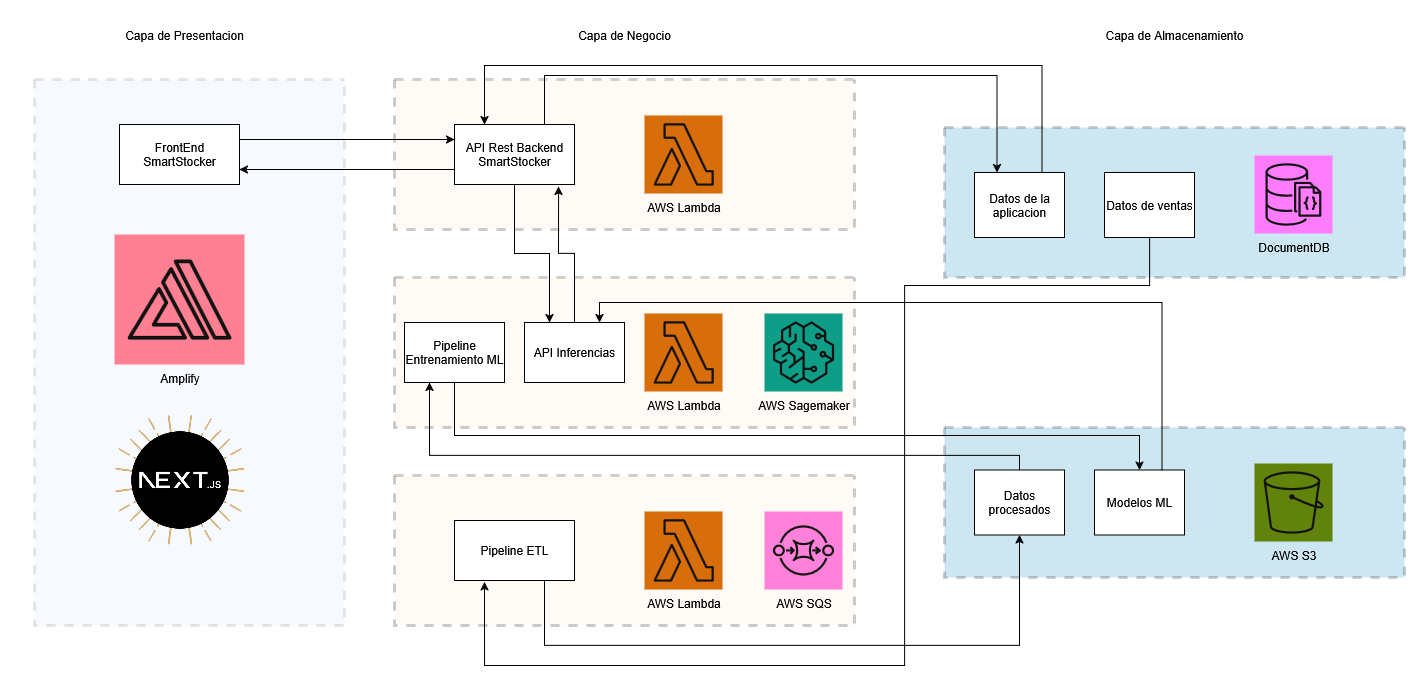
\includegraphics[width=0.7\textwidth]{images/arquitectura_capas.png}
    \caption{Arquitectura conceptual de SmartStocker}
    \label{fig:arquitectura-conceptual}
\end{figure}

\subsection{Diagrama de Despliegue}\label{sec:arquitectura-despliegue}
Se decidió usar Amazon Web Services (AWS) como solución de despliegue para nuestra solución, debido a la flexibilidad y amplitud de herramientas ofrecidas necesarias para implementar la arquitectura de SmartStocker.

Analizando la capa de presentación, esta se encuentra desarrollada con Next.js, y desplegado a través de AWS Amplify. Se eligió este servicio puesto que simplifica enormemente la gestión de la aplicación, permitiendo, mediante una simple configuración inicial, encargarse de aspectos tales como el despliegue (permitiendo CI/CD integrado a GitHub), hasta del escalamiento en sí.

Para la capa de almacenamiento, se optaron por dos soluciones. Primero, DocumentDB como base de datos NoSQL, seleccionado debido a la naturaleza no estructurada de los datos a utilizar, y que nos brinda la posibilidad de modificar el schema con facilidad, además de ser una base serverless escalable. Y segundo, S3, para contener la información en formato \verb|csv| requerida para los entrenamientos del modelo, y para almacenar los archivos correspondientes al modelo entrenado en si.

Para la capa de negocio, se decidió implementar las distintas APIs requeridas mediante AWS Lambda, dado que su enfoque serverless permite abstraernos de la gestión de la infraestructura, acelerando el desarrollo y la puesta en producción, escalando cuando la demanda lo requiera, y reduciendo los costos fijos.

Esto también aplica para el pipeline de ETL, donde también se utiliza AWS Simple Queue Service (SQS) para desacoplar el procesamiento de las ventas, a fin de lograr velocidades de respuesta rápida ante los sistemas externos que enviaran las mismas, mientras que el procesamiento y enriquecimiento de las ventas se realiza en otra Lambda.

Por último, se decidió usar AWS Sagemaker en el pipeline de ML, puesto que simplifica enormemente el entrenamiento del modelo, requiriendo suministrarle solamente el dataset a utilizar, y permite disponibilizar el modelo para ser usado para predicciones mediante endpoints, lo que brinda una consulta rápida y de facil implementacion.

\begin{figure}[htbp]
    \centering
    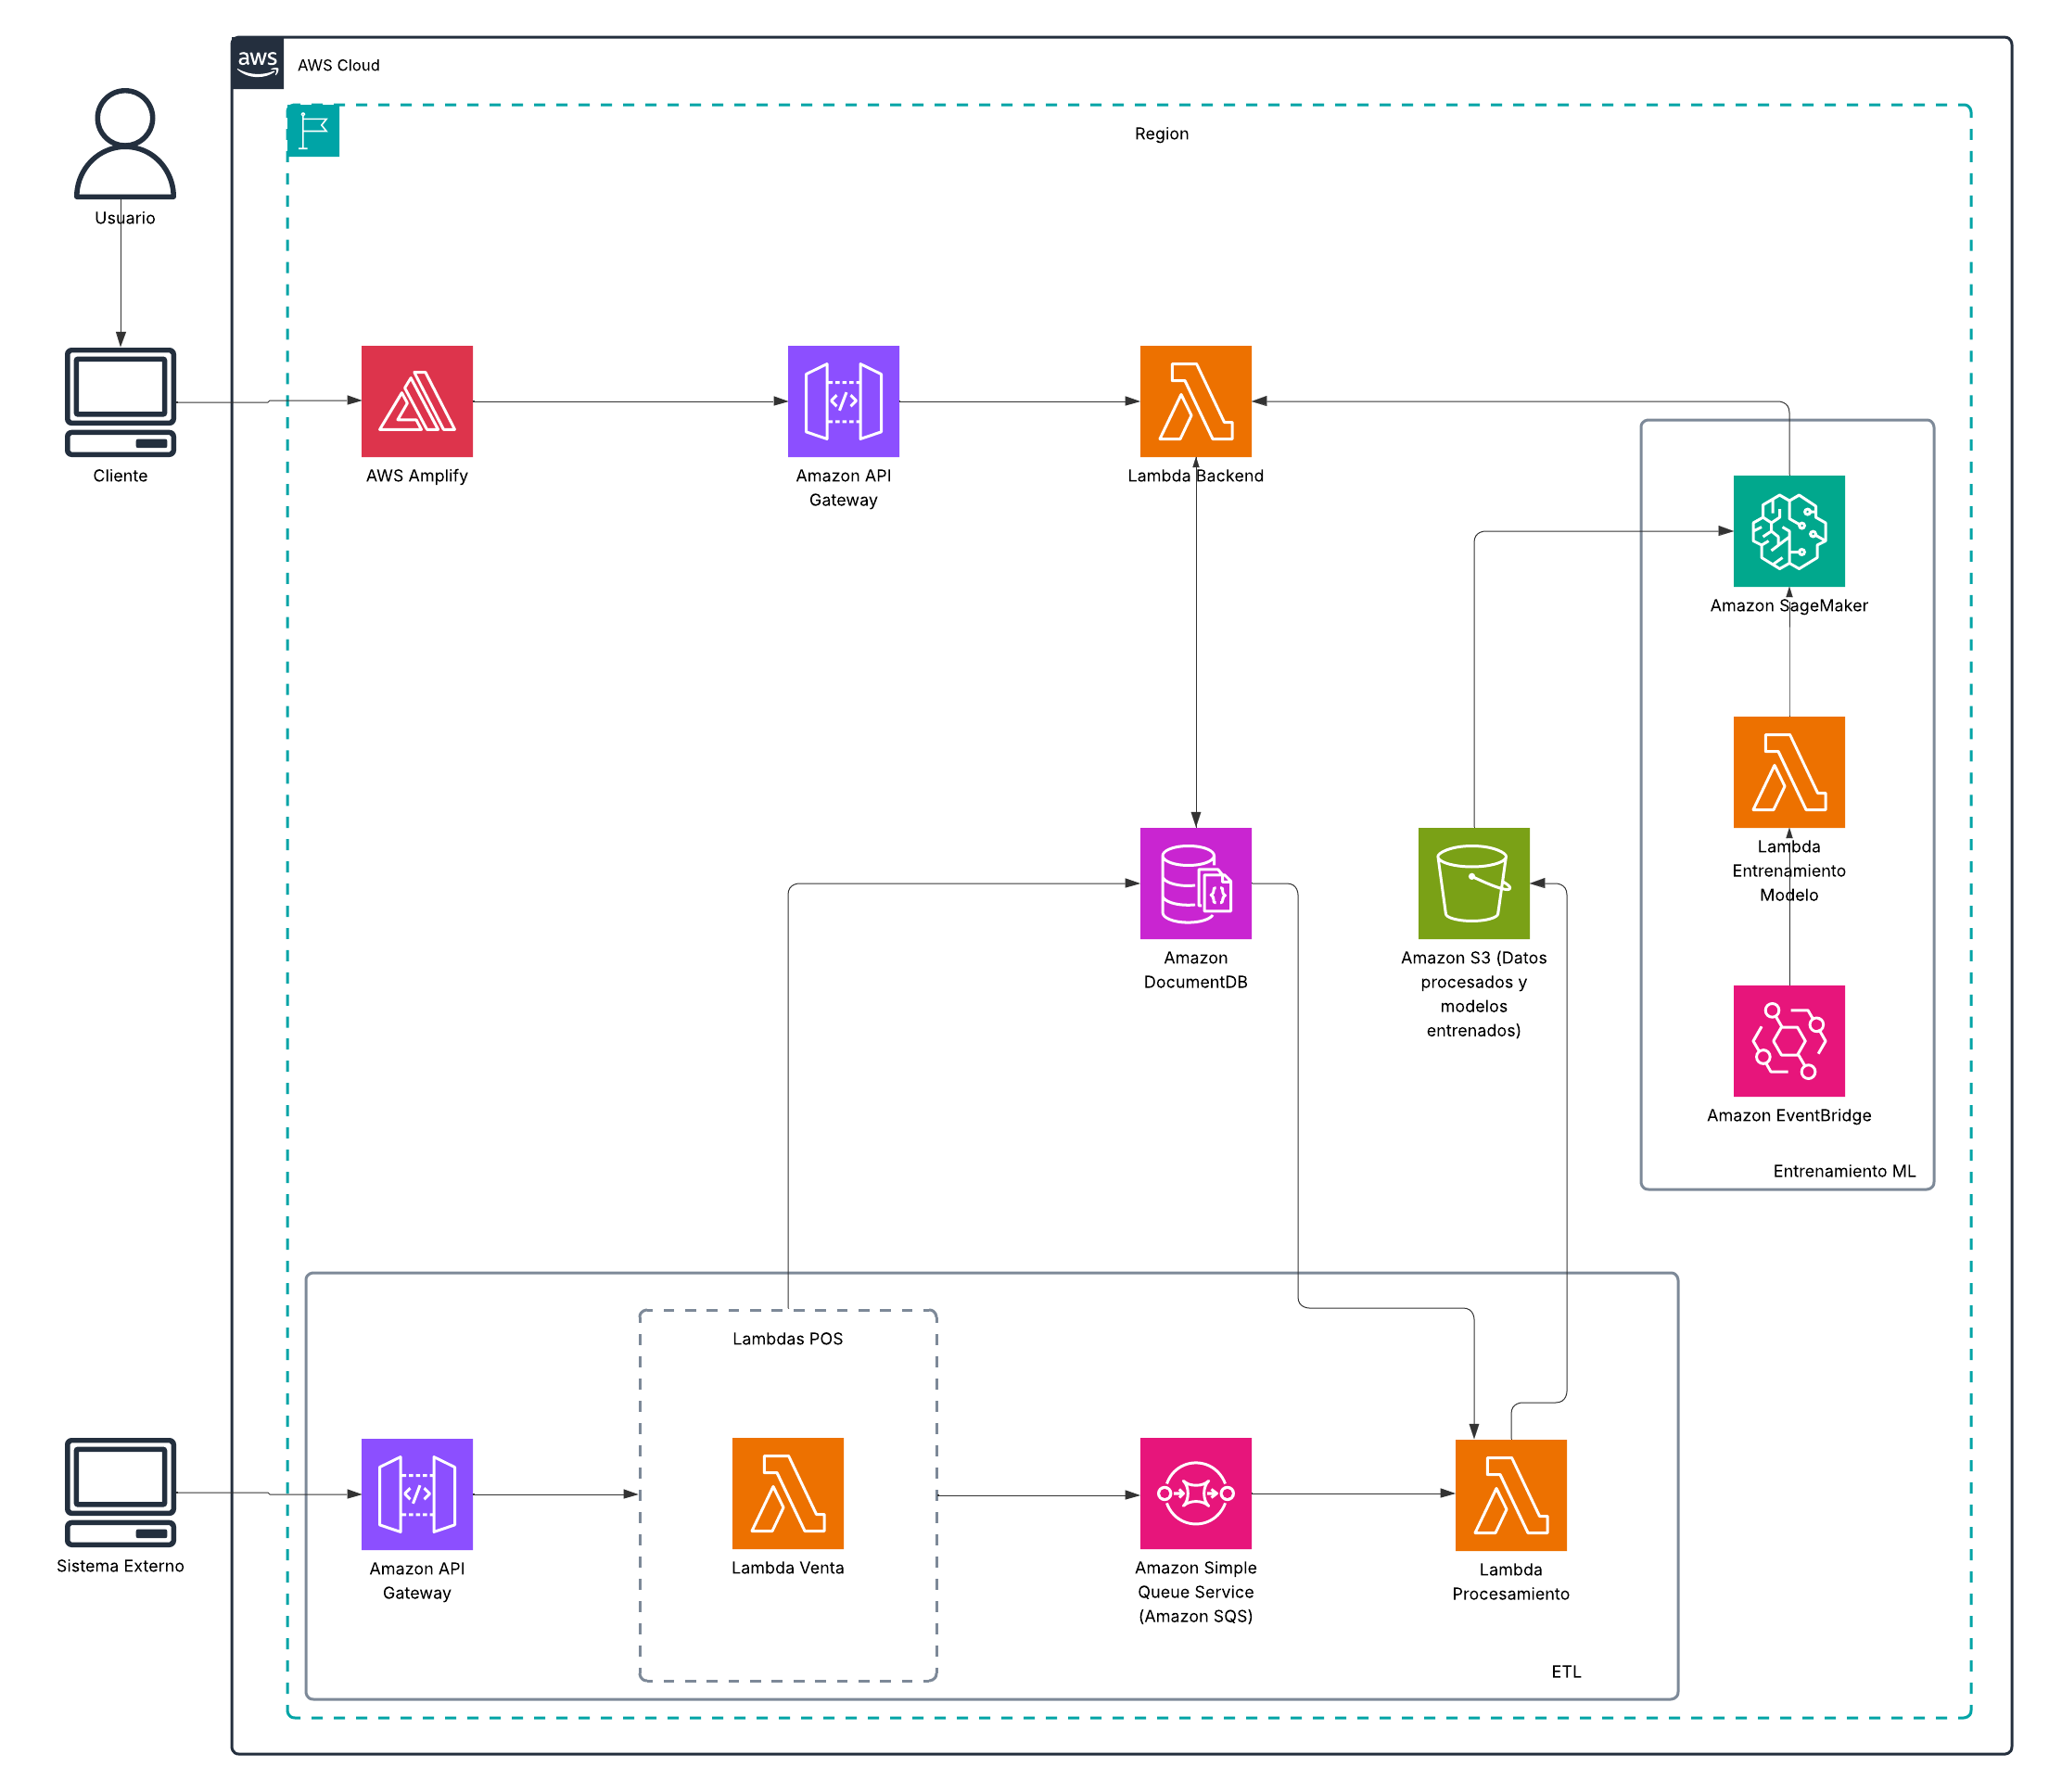
\includegraphics[width=0.7\textwidth]{images/arquitectura_despliegue.png}
    \caption{Arquitectura de Despliegue y Procesos de SmartStocker}
    \label{fig:arquitectura-despliegue}
\end{figure}

\subsection{Diagrama de Base de datos}\label{sec:arquitectura-base-datos}

Para el diseño de la base de datos, se opto por utilizar DocumentDB, una de las alternativas NoSQL brindadas por AWS, debido a la flexibilidad y capacidades de escalado automatico que esta nos provee, siendo la flexibilidad del schema algo critico dada la necesidad de agregar campos adicionales conforme el proceso de ETL o entrenamiento del modelo de ML lo requieran.

El diseño de la base de datos se organiza alrededor de cinco entidades principales: Usuario, ItemMenu, Ingrediente, Predicción y Venta. La entidad Usuario representa a un negocio dentro de la plataforma. A su vez, la entidad Ingrediente almacena los insumos (nombre, unidad de medida, cantidad en stock y cantidad mínima) y su propietario (userId), mientras que ItemMenu registra los productos ofrecidos (código, nombre, estado activo) y contiene la lista de ingredientes necesarios para cada receta. Esa relación N:M entre ItemMenu e Ingrediente se materializa en la tabla/intersección (el subdocumento de ingredientes) que guarda, por cada par producto-ingrediente, la cantidad\_requerida. La entidad Predicción registra las predicciones de demanda vinculadas a un producto\_id (ItemMenu) con fecha\_prediccion, turno, cantidad\_predicha y el userId que la generó; y la entidad Venta recoge las transacciones reales (número de venta, ítem, producto, cantidad, precio unitario, subtotal, fecha, turno, plataforma, método de pago y estado) asociadas también a un userId. Todos los documentos incluyen timestamps (fecha\_creacion / fecha\_actualizacion) para auditoría.

\begin{figure}[htbp]
    \centering
    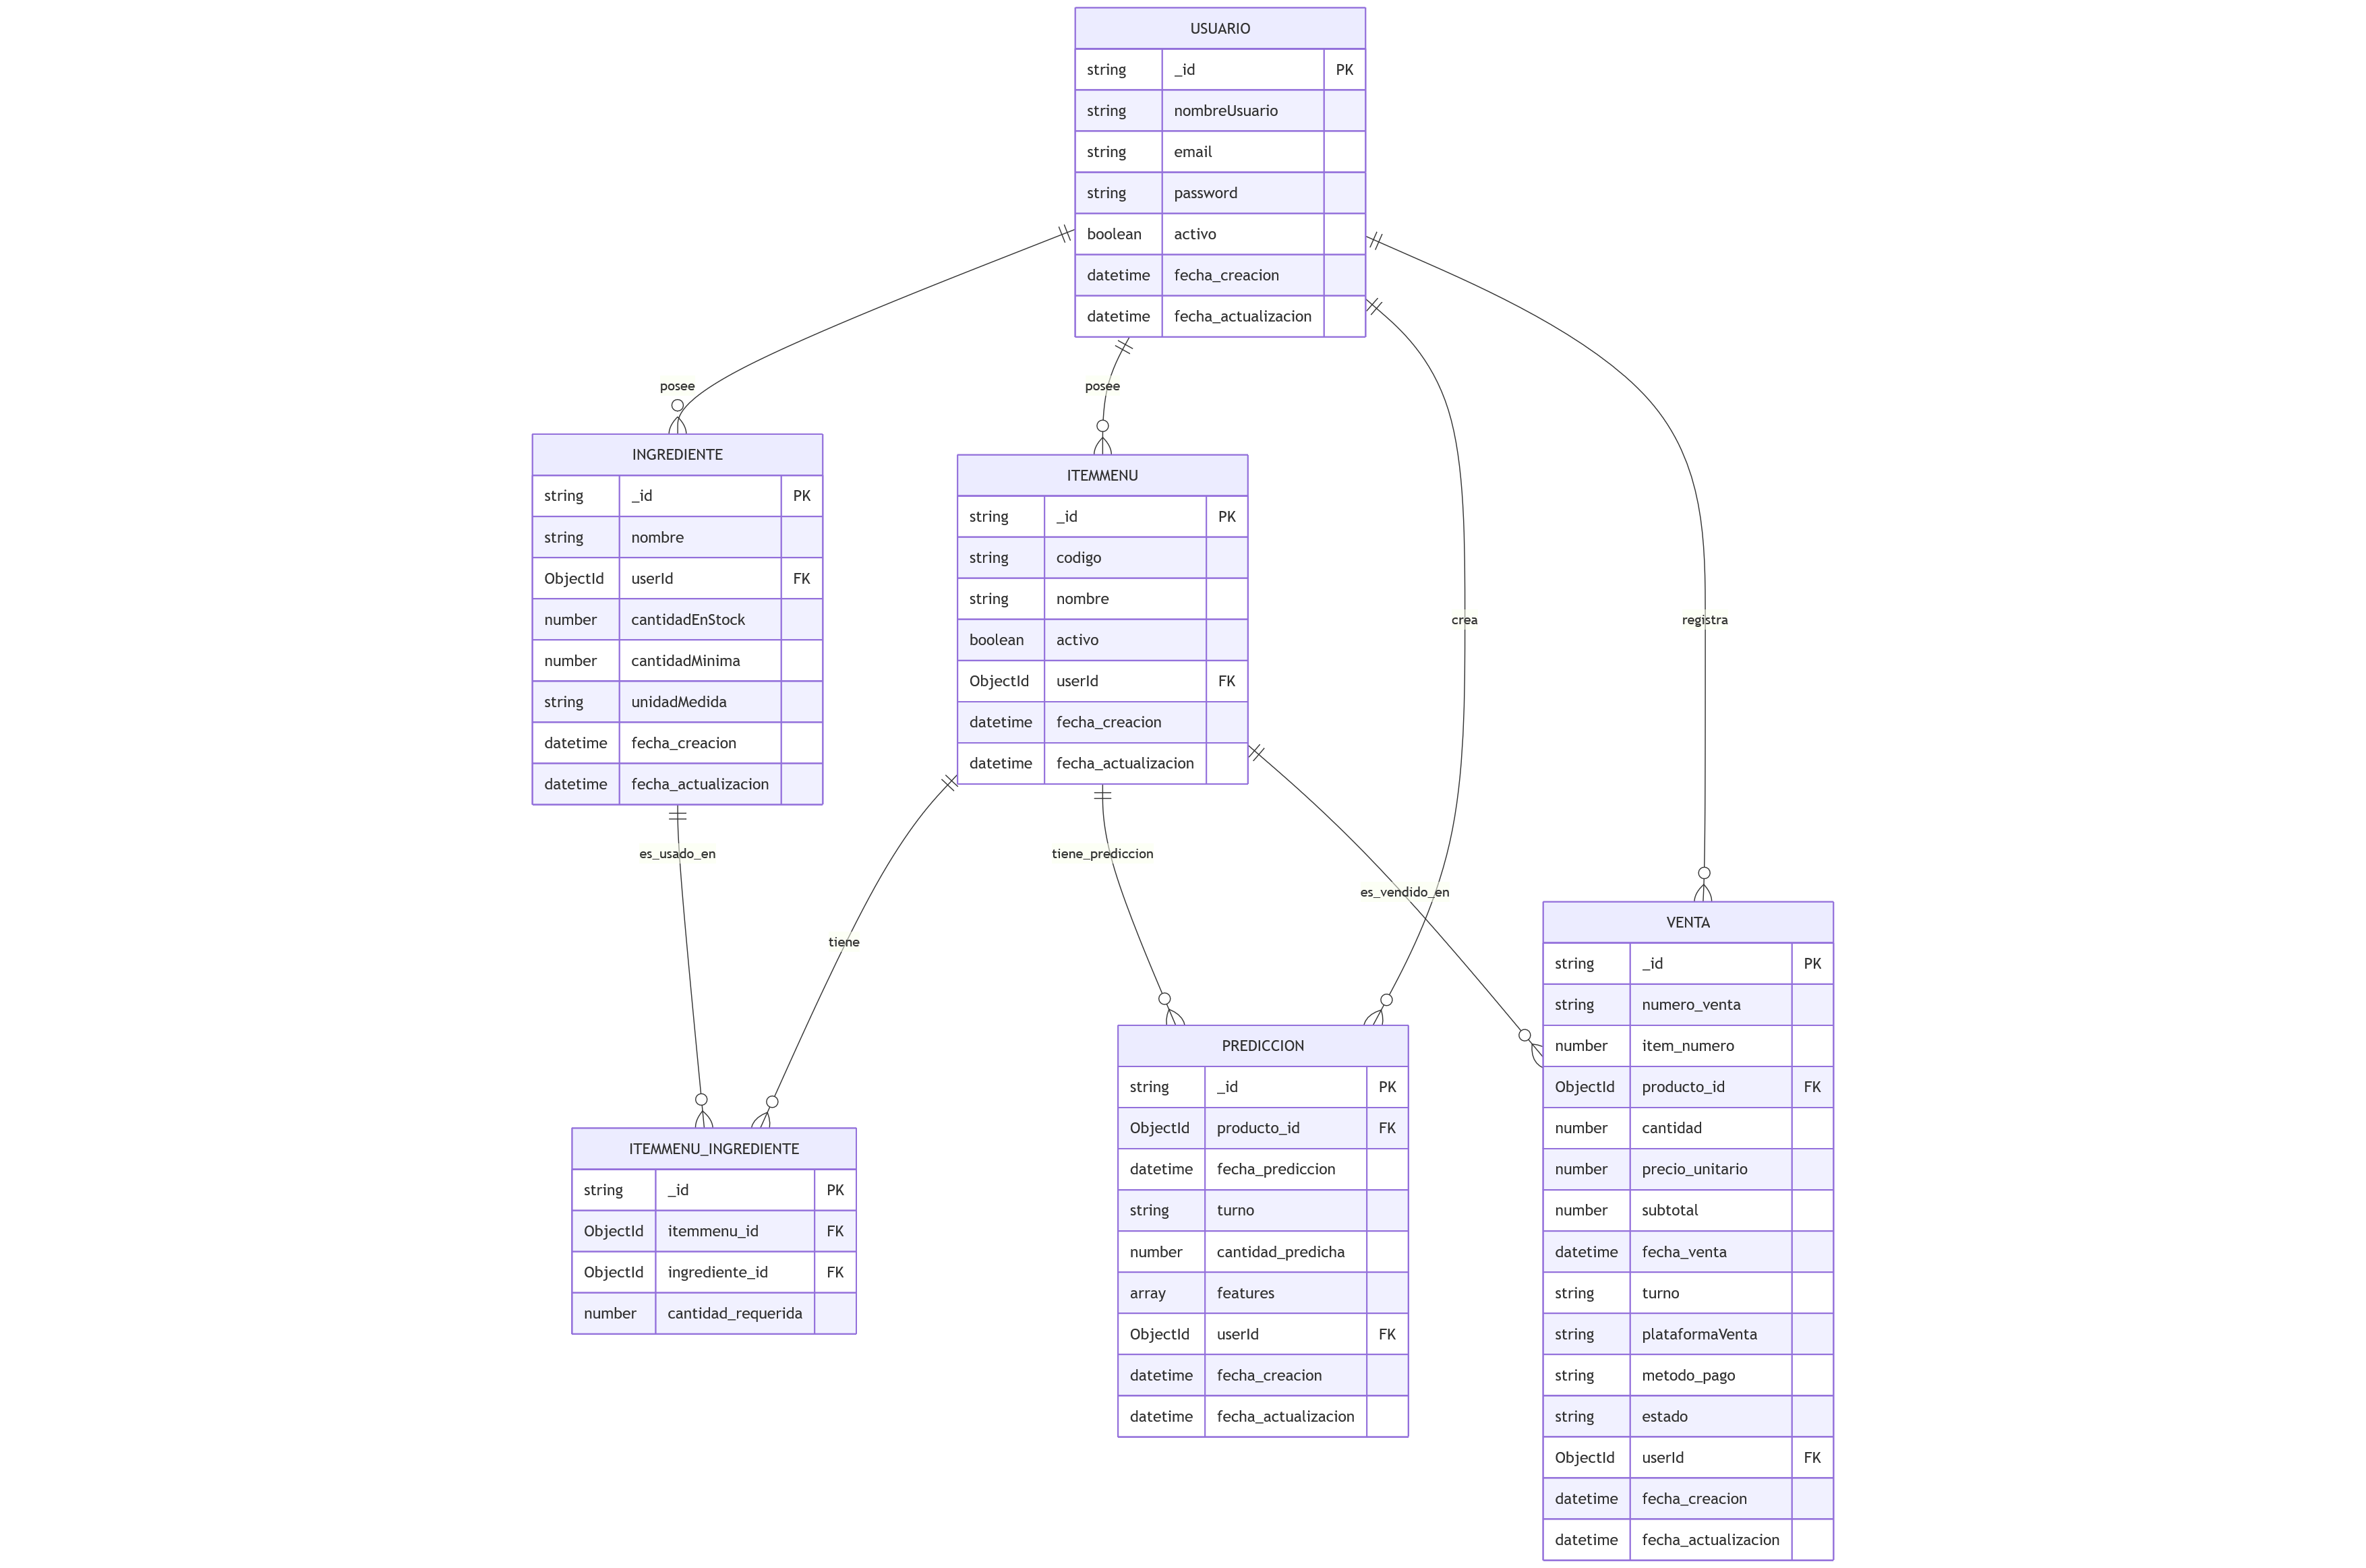
\includegraphics[width=0.7\textwidth]{images/arquitectura-base-datos.png}
    \caption{Arquitectura de Base de Datos de SmartStocker}
    \label{fig:arquitectura-base-datos}
\end{figure}

\subsection{Pipeline ETL}\label{sec:pipeline-etl}

Con el objetivo de permitir la ingesta automática de las ventas, a fin de actualizar tanto los dashboards visualizados en la aplicación, activar las correspondientes alertas de stock si fuera necesario y disponibilizar la información para el entrenamiento del modelo predictivo, se implementó un pipeline de ETL mediante el cual se procesan las distintas ventas. La primera parte de este proceso es recibir y procesar las ventas que ocurren, para lo cual se diseñaron distintas Lambdas, ajustadas al distinto formato en el que las plataformas pueden enviar los datos de una venta realizada. En estas se analiza la información recibida y en base a ello se genera una nueva entrada en la entidad Ventas. Dado que estas Lambdas estarán atendiendo peticiones de sistemas externos, se decidió que el procesamiento que ocurre en ellas sea lo más rápido y sencillo posible, a fin de devolver una respuesta a la brevedad.

En base a esto, se implementó el uso de AWS SQS, permitiendo de esta forma que el resto de procesamiento requerido para transformar la venta en el dato requerido por el modelo ocurra en una Lambda distinta, que funciona como consumidor de la cola implementada en SQS, donde al finalizar la primer Lambda se encola un mensaje conteniendo el Id de la venta creada en DocumentDb, para que esta sea procesada por el consumidor. Esto nos brinda un procesamiento asincrónico y desacoplado de estas tareas que pueden ser más lentas, y permite que ocurran a un ritmo distinto de la Lambda inicial expuesta al resto de los sistemas de venta.

Esta segunda Lambda se encargará de, en base a la información de la venta y consultas a APIs externas para la obtención de feriados y datos climáticos, generar las features que se considerarán en el entrenamiento del modelo, donde se consideran aspectos relacionados al momento cronológico de la venta, es decir, en qué turno de trabajo ocurre, si se realizó en un feriado, en que semana se hizo, si la venta ocurrió en un fin de semana, pero también se considera el aspecto climático, indicando tanto la estación como el estado climático en ese momento (nublado, despejado, lluvioso), a fin de lograr aspectos estacionales del consumo.
Por último, al finalizar esta Lambda la información procesada es almacenada en un S3, disponible para ser usada al momento de entrenar el modelo.


\subsection{Pipeline Machine Learning}\label{sec:pipeline-machine-learning}

El pipeline de entrenamiento del modelo de machine learning se encuentra implementado mediante el uso de AWS EventBridge, a fin de programar entrenamientos periódicos de forma semanal. El EventBridge disparará un evento que activará una Lambda dedicada al entrenamiento, donde se harán los últimos ajustes a los datos de entrenamiento, se consolidaran los datos de venta, unificando las distintas ventas individuales de acuerdo a la fecha, turno, y producto y se programará la ejecución del entrenamiento en sí, utilizando para esto AWS Sagemaker. Luego del entrenamiento, el modelo será disponibilizado a través de un endpoint, accesible desde la API del backend de la aplicación.

\subsection{Inclusión del Feedback de usuario}\label{sec:inclusion-feedback-usuario}

A fin de incluir el feedback del usuario dentro de las predicciones, se decidió la inclusión de un segundo modelo, cuyo propósito será ajustar la salida del modelo principal, considerando, para cada combinación de producto, turno, y fecha: 

\begin{itemize}
    \item la cantidad de ventas predecida por el modelo.
    \item la cantidad de ventas que efectivamente ocurrieron.
    \item la cantidad de ventas que el usuario espera, brindado como feedback.
\end{itemize}

Este modelo será utilizado para ajustar únicamente las predicciones de productos en las cuales el usuario haya brindado algún feedback, usando únicamente el modelo principal para el resto de productos. Su entrenamiento ocurre en un pipeline similar al del modelo principal, usando como datos de entrenamiento los descritos previamente. A la hora de ejecutar las predicciones, en caso de que haya productos que han recibido feedback por parte del usuario de forma reiterada, esta predicción original será pasada por el segundo modelo, a fin de ajustarla.
